\documentclass{article}
\usepackage[]{graphicx}
\usepackage[]{xcolor}
\usepackage{alltt}
\usepackage[left=2.3cm,right=2.8cm, top = 2.2cm, bottom = 3cm]{geometry}
\usepackage{amsmath}
\usepackage{amssymb}
\usepackage{natbib}
\PassOptionsToPackage{hyphens}{url}
\usepackage{url} 
\usepackage[disable]{todonotes}
\usepackage{multicol}
\usepackage{rotating}
\usepackage{booktabs}
\usepackage[colorlinks=false]{hyperref} 
\setlength{\parskip}{\baselineskip}%
\setlength{\parindent}{0pt}%
\urlstyle{same}
\usepackage{lineno}
\linenumbers


% to handle authorship footnotes as numbers:
\makeatletter
\let\@fnsymbol\@arabic
\makeatother

\newcommand{\ra}[1]{\renewcommand{\arraystretch}{#1}}
\newcommand{\changed}[1]{#1}


\begin{document}


\title{To log or not to log}
  \author{Anonymous Alpaca\thanks{All Alpaca friends} $^{,}$\thanks{The Zoo} $^{ , *}$}

\maketitle

\tableofcontents

\begin{abstract}
In the abstract, this article is a very good one. We did a very good job of the research and got all the best results. People told us we were mad and we said no we are effective. Now gather around and listen to our thoughts you will be, shocked, scared, amazed, and astounded.
\end{abstract}

\bigskip

{\footnotesize $^*$ Correspondence to: Anonymous Alpaca (\url{anonymous@alpaca.com}))}



\newpage


% ===========================================================
\section{Introduction}

Probabilistic forecasts play an important role in decision-making in epidemiology and public health [Citations], as well as other areas as diverse as for example economics [Citations] or agriculture [Citations]. Epidemiological modelling in particular has received widespread attention during the COVID-19 pandemic and has been an important tool to inform public policy. Evaluating forecasts is important, as the evaluation provides feedback for forecasters and researchers necessary to improve their models, and it helps decision makers with distinguishing good from bad predictions and choosing forecasts that inform future decisions.

Proabbilistic forecasts are usually evaluated using so-called proper scoring rules, which return a numerical score as a function of the forecast and the later observed data. Forecasters, in expectaction, optimise their score by providing a predictive distribution that is equal to the data-generating distribution, and will be penalised if they fail to do so. Two proper scoring rules commonly used in epidemiology and other fields are the Continuous Ranked Probability Score (CRPS) [Gneiting 2007] and the Weighted Interval Score (WIS) [CITATION]. Due to their widespread use we focus on these two in this paper, ignoring other proper scoring rules. Both the WIS and CRPS represent a measure of the absolute distance between the predictive distribution and observation and can be thought of as a generalisation of the absolute error to full predictive distributions (see details in the SI). 

Evaluating forecasts based on absolute errors (for simplicity we use the term interchangeably with absolute distance, even though it technically only applies to point forecasts) may not always be desirable, especially in an epidemiological context. 
% The reason for this is that generally, the way forecasts are evaluated should correspond to the error structure of the model and the type of errors models will usually make.
Epidemiological processes are usually understood to be exponential in nature and therefore are most commonly described and modeled in multiplicative terms. Under the assumption that these models are correctly capturing the underlying inherent transmission dynamics, it would therefore make sense to focus evaluation on multiplicative, rather than absolute errors. Often, if the model is performing badly in multiplicative terms, this means that there is a flaw with its assumptions that needs to be resolved, regardless of performance in absolute terms. Evaluating epidemiological forecasts based on a measure of absolute error (as is common practice) can make it harder to diagnose and quantify model mis-specification. It also may make it more difficult to deal with the potential non-stationarity of epidemiological processes, or to compare performance across targets that are on very different orders of magnitudes (like for example cases and hospitalisations). 

In this paper we argue that it may therefore often be helpful to shift the focus of the evaluation on multiplicative, rather than absolute errors. This can be achieved by transforming the forecasts as well as the observations using the logarithm before applying the WIS or CRPS. While we will mostly focus on the log transformation in this paper, the point we like to make is a broader one: it is possible to flexible change the focus of the evaluation by applying a multitude of different transformations before scoring forecasts. Instead of scoring multiplicative errors, one may for example like to apply a transformation that allows to score forecasters based on the shape of the trajectory they predicted. Furthermore, it is possible to capture different aspects in a single number by constructing composite scores as a weighted sum of scores based on different transformations. This allows forecast consumers to assign explicit weights to different qualities of the forecasts they deem to be important when assessing predictive performance. 

In section [REF] we discuss which kinds of transformations can be applied. In section [REF] we give a detailed theoretical explanation of the rationale for applying the log transformation and discuss its interpretation. In section [REF] we present an applied example using forecasts submitted to the European COVID-19 Forecast Hub. The European COVID-19 Forecast Hub is one of several Forecast hubs (together with a Hub in the US [CITATION] and one in Germany and Poland [CITATION]) that systematically collected, aggregated and evaluated forecasts of several COVID-19 targets created by different teams. Forecasts submitted to the COVID-19 Forecast Hubs are probabilistic in nature [Citation e.g. Held et al.], meaning that forecasters provide a full predictive distribution which quantifies their uncertainty. These predictive distributions are reported in the form of a set of 23 quantiles (11 symmetric prediction intervals as well as a median prediction). 
%Currently, the US Flu Forecasting Hub and COVID-19 Scenario Hubs in the US and in Europe use the same format. 

%%%%%%%%%%%%%%%%%%%%%%%%%%%%%%%%%%%%%%%%%%%%%%%%%%%%%%%%%%%%%%%%%%%%%%%%%%%%
\section{Transforming forecasts to shift the focus of the evaluation}

\subsection{Permissible transformations / propriety} - JOHANNES

In order to preserve the propriety of the score, transformations must be strictly monotonic. This makes sure that a forecast that is further away from the observed value will also be further away after the transformation. 

- WHAT KINDS OF DATA CAN I CONDITION ON? 
- WOULD DIVIDING A FORECAST BY ITS RESOLUTION WORK? 
- CAN I SCORE THE TRAJECTORY / WEEK-TO-WEEK GROWTH RATE BY DIVIDING the 4 week ahead forecast by the three week ahead forecast? 
Probably does not work. 
Problem: Median von (X\_t+4 / X\_t+3) ist anders als Median 

\paragraph{First transform, then score, rather than the other way round}
Note that simply taking the log of a score computed on the natural scale, i.e. computing $\log S(x, y)$ results in an improper score and is therefore not advised. We illustrate this point in Figure \ref{fig:log-improper} in the SI. 

% \paragraph{Changes only come when you average across multiple scores}
% For a single forecast, the ranking between forecasters would be preserved and the scores remain proper [Proof?]. Differences in the ranking between forecasters only appear when averaging over multiple forecasts, as deviations from the perfect forecast get penalised differently depending on whether forecasts are transformed or not. 

\paragraph{Example transformations}

Take the log

Divide by the latest known value = score forecast on the growth rate

Log that = score log growth rate

Divide by the previous for each time value, which gives you a weekly growth rate, i.e. a trajectory. 

Box-Cox

square root WAS THAT USED SOMEWHERE? This is stabilising the variance. Kraus und Kraus. Idea: if X is poisson with some mean, then sqrt(x) has asymptotically a constant variance

Standardising by population size

%%%%%%%%%%%%%%%%%%%%%%%%%%%%%%%%%%%%%%%%%%%%%%%%%%%%%%%%%%%%%%%%%%%%%%%%%%%%
\section{Log transforming forecasts and observations}

In this section (and those that follow) we focus on one particular transformation, taking the logarithm of forecasts and observations, which makes it possible to change the focus of the evaluation from absolute to relative errors. To illustrate the effects of applying the logarithm intuitively, let us consider a point forecast $\hat{y}_{t+1}$ for a quantity of interest $y_{t+1}$, such that 
\begin{equation}
y_{t+1} = \hat{y}_{t+1} + \varepsilon_{t+1}.
\end{equation}

The analogon of the WIS / CRPS for point forecasts is the absolute error, and so the score will be determined by the size of the forecast error $\varepsilon_{t+1}$. When taking the logarithm of the forecast and the observation first, than the score is determined based on the size of $\varepsilon^*_{t+1}$: 
\begin{equation}
\log y_{t+1} = \log \hat{y}_{t+1} + \varepsilon^*_{t+1}.
\end{equation}
%
It is easy to see that this corresponds to evaluating a multiplicative error on the original $y_{t+1}$:
%
\begin{align}
\log y_{t+1} &= \log \hat{y}_{t+1} + \varepsilon^*_{t+1} \Leftrightarrow \\    
y_{t+1} &= \hat{y}_{t+1} \cdot \exp{\varepsilon^*_{t+1}}.    
\end{align}
%

On the natural scale, WIS and CRPS increase linearly with increasing absolute errors (see Figure \ref{fig:change-in-scores}A, regardless of whether the error is large in relative terms. Predicting 101,000 cases instead of the true 100,000 will be treated equally to predicting 2,000 hospitalisations, rather than the 1,000 observed. On the log scale, WIS and CRPS penalise relative errors and increase linearly with an increase in relative errors (see Figure \ref{fig:change-in-scores}D). Forecasting 101,000 rather than 100,000 cases will be treated equally to forecasting 2,020, rather than 2,000 hospitalisations. 
% Note that for a single forecast the relative rankings of different forecasts would be preserved. The transformation only makes a difference when aggregating predictions across different dimensions. 

\begin{figure}[h!]
    \centering
    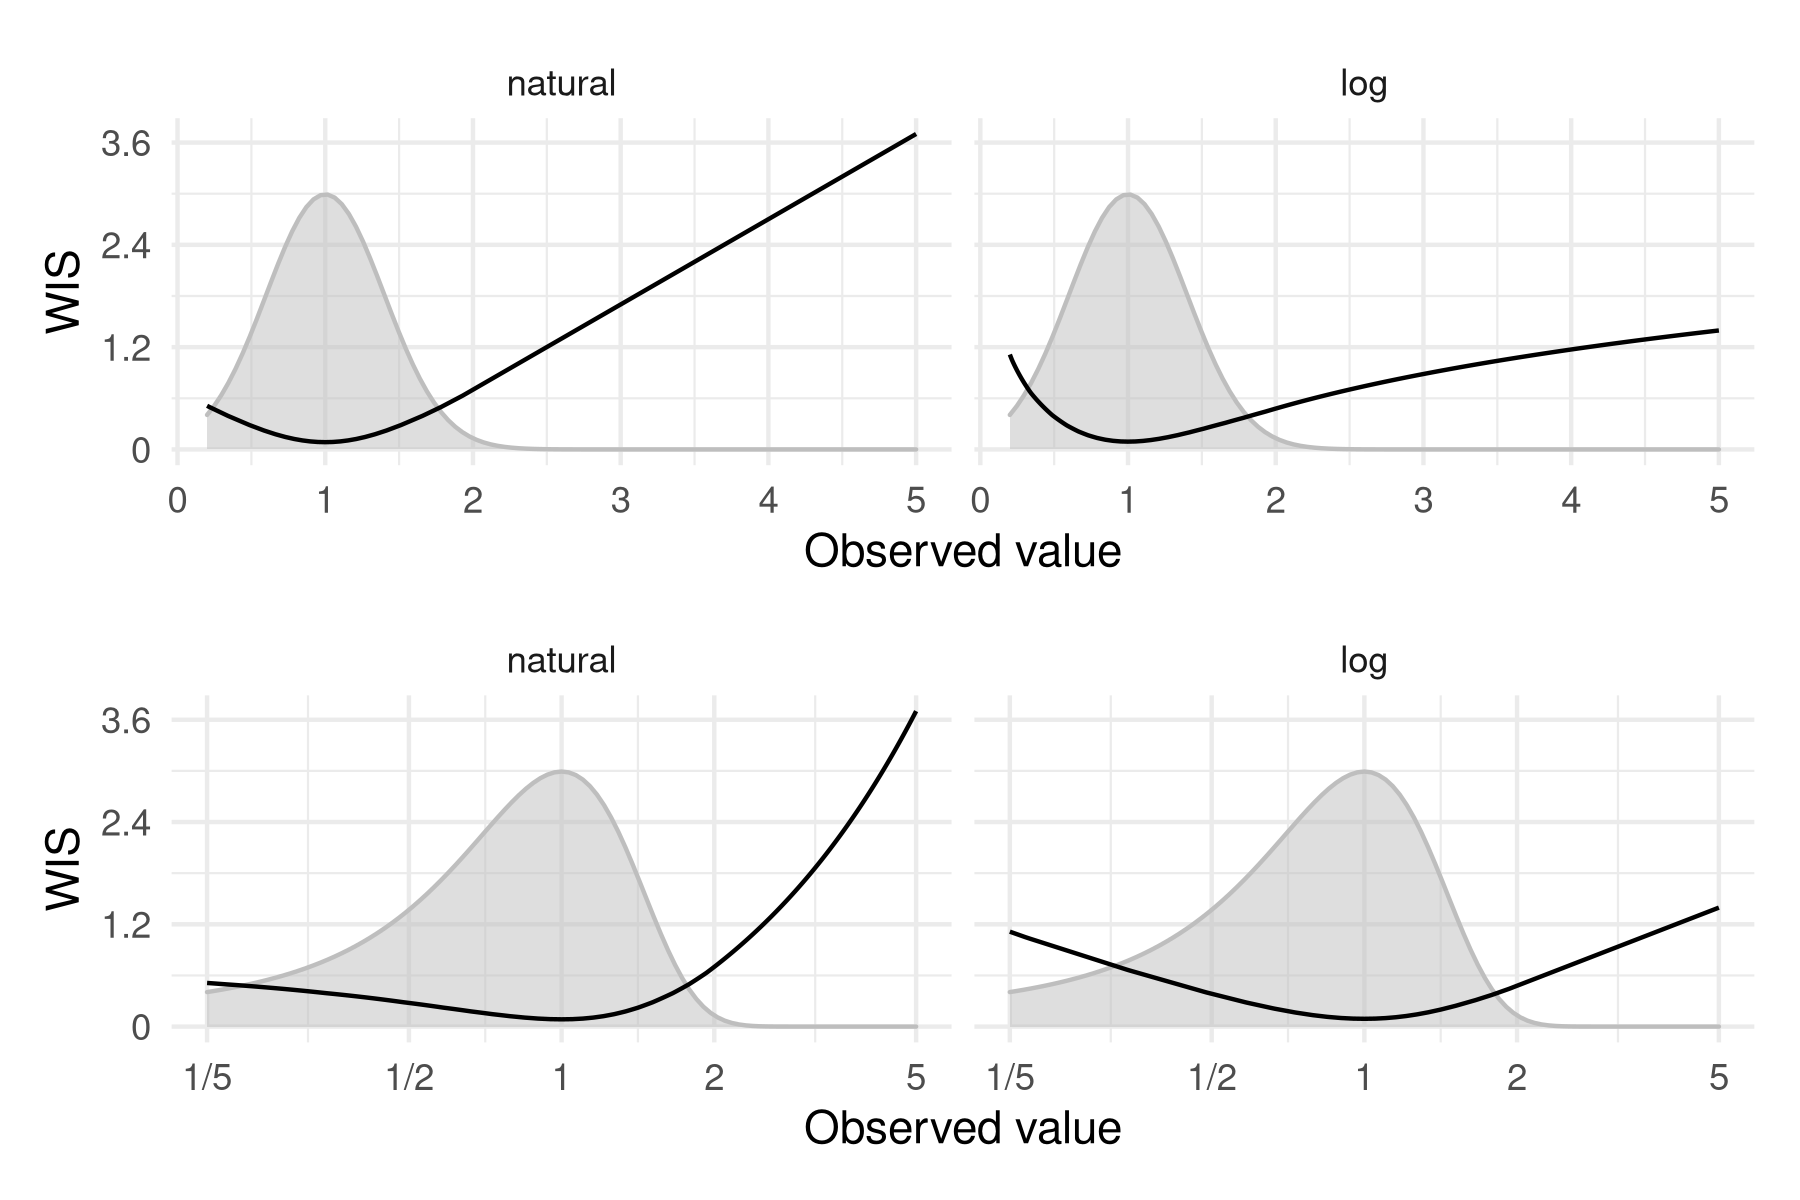
\includegraphics[width=0.9\textwidth]{output/figures/SIM-effect-log-score.png}
    \caption{Weighted interval score for a forecast distribution that is N(1, 0.2) and different observed values. Top: difference in absolute terms. Bottom: difference in relative terms. Interesting panels are top left and bottom right.} 
    \label{fig:change-in-scores}
\end{figure}

\subsection{Approximately scoring the growth rate}
Computing a score based on the logarithm of the forecast and the observation is also approximately equivalent to scoring a forecast of a multiplicative growth rate of the forecast target. The growth rate is defined as
%
\begin{equation}
    g_{t, t+1} = \frac{y_{t+1} - y_t}{y_t},
\end{equation}
%
where $y_{t+1}$ is the forecast target (e.g. reported cases of COVID-19) in the future, $y_t$ is the last known observation and $g_{t, t+1}$ is the growth rate between now ($t$) and $t+1$. 
Using the growth rate, we can express the value of the forecast target in the future as such: 
%
\begin{equation}
y_{t+1} = (1 + g_{t, t+1}) \cdot y_t.
\end{equation}
%

Now consider a forecast on $\log y_{t+1}$. Using the fact that for small values of $x$, $\log (1+ x) \approx x$, we can see that scoring forecasts on the log scale is approximately equal to scoring an additive error on the growth rate (on the natural scale), as long as the growth rate is small.
%
\begin{align}
\log y_{t+1}        &= \log \hat{y}_{t+1} + \varepsilon^*_{t+1} \\
                    &= \log ((1 + \hat{g}_{t+1}) \cdot y_{t}) + \varepsilon^*_{t+1} \\
                    &= \log (1 + \hat{g}_{t, t+1}) + \log y_t + \varepsilon_{t+1} \Leftrightarrow \\
\varepsilon'_{t+1}  &= \log y_{t+1} -  \log y_t - \log (1 + \hat{g}_{t, t+1}) \Leftrightarrow \\    
                    &= \log (\frac{y_{t+1}}{y_t}) - \log (1 + \hat{g}_{t, t+1}) \Leftrightarrow \\    
                    &= \log (1 + g_{t, t+1}) - \log (1 + \hat{g}_{t, t+1}) \Leftrightarrow \\   
                    &\approx g_{t, t+1} - \hat{g}_{t, t+1} \quad \text{for small } \hat{g}_{t, t+1}, g_{t, t+1}. 
\end{align}

%maybe it suffices that the difference between them is small. You can write them as a ratio and then the ratio just needs to be similar to one. 

This approximation breaks down when the growth rate becomes too large. If scoring the growth rate is the focus of the evaluation, then it may be better to transform forecasts and observations by the last known values instead in order to score the growth rate explicitly. 

\subsection{Dealing with negative counts and small values}
Unfortunately, the log transformation cannot readily be applied when dealing with negative or zero values. In an epidemiological setting that involves count data, negative values should likely be omitted entirely. Values of zero should potentially also be removed from the analsys, as it does not make sense to interpret relative errors on zero counts. Alternatively, if one is not willing to omit them, a small quantity (such as 1) could be added to all observations before taking the logarithm. Note that predictive distribtions have to be truncated in a similar way. When dealing with count data we could extend this argument to all small values (rather than just zeros), as it is hard to reliably evaluate relative errors when dealing with small discrete values. One could therefore decide to remove forecasts for small quantities below a certain threshold from the analysis. Alternatively, one could add a number $n$ (e.g. $n = 100$) to all observations and forecasts before taking the logarithm. This constitutes a strictly monotonic transformation which preserves propriety and would reduce all scores (through reducing relative errors). Scores for forecasts on small quantities would be particularly affected, resulting in a more equal distribution of scores for forecasts of differing orders of magntitudes. Researchers can choose to add either a small or large number, depending on how much they want to equalise relative errors when aggregating scores. 

\subsection{Relative importance when summarising scores}
% Stationarity of forecast timelines

For a single transformation, the ranking between models is preserved, even though the numeric value of the score changes. However, when averaging across forecasts, the relative influence of individual forecasts on the aggregate score may differ dramatically, leading to changes in the overall model rankings. While the main rationale for applying the log transformation is that this better reflects the types of errors common in epidemiological modelling, it may also be helpful when scores based on the natural scale are very unequal. This usually happens, for example, when different forecast targets, like reported case numbers, hospitalisations and deaths, or the same targets across time and space, have very different orders of magnitude. In these instances, scores (even for an ideal forecaster) usually also differ by several orders of magnitude. Evaluating forecasts based on relative errors often makes it easier to compare performance across different targets more easily (as scores of an ideal forecaster would not differ as much as on the natural scale). 

While on the natural scale, aggregate scores will usually be dominated by predictions of quantities with high absolute values, the opposite may be true for scores based on log transformed predictions. Small absolute errors (e.g. predicting 9, rather than 3 deaths) may be large in relative terms if the quantity to forecast is very small. The strength of this effect depends on the exact relationship between the mean and the variance of the quantity of interest. For simulated negative binomial count data, log predictions for small quantities receive on average higher scores than forecasts for large quantities if the mean and the variance grow at the same rate $\sigma^2 = \mu$, about equal scores when the variance grows at a rate of $\sigma^2 = \mu + \mu^2$ (Figure \ref{fig:SIM-wis-state-size-mean}), and smaller scores when the variance grows faster than that. As mentioned above, one way to handle situations where scores are very unequal, is to add a number $n$ to all forecasts and observations in order to reduce the relative weight of forecast targets with small quantities. 


% To illustrate this with count data we sampled forecasts from different negative binomial distributions. The negative binomial distribution has mean $\mu$ and variance $\sigma^2 = \mu + \mu ^2 / \theta$ and for $\lim_{\theta \to \infty}$ converges to the Poisson distribution. For large values of $\theta$, resulting in a variance approximately equal to the mean, forecasts for lower quantities on average received higher scores on the log scale (see Figure \ref{fig:SIM-wis-state-size-mean}. For $\theta = 1$ (and correspondingly, $\sigma^2 = \mu + \mu^2$, we found that scores on the log scale remained approximately constant regardless of the size of the quantity to forecast. For $\theta = 0.1$ (and $\sigma^2 = \mu + 10 \cdot \mu^2$), scores on the log scale increased with the quantity to forecast. When scored on the natural scale, a higher quantity to forecast always lead to higher scores regardless of the chosen distribution (as long as the variance grows together with the mean). 


COULD ALSO BE DISCUSSION
Whether or not a log transformation is apprpriate depends on whether one believes that differences in absolute values are meaningful. This may be the case for example when comparing forecasts across locations or time points, rather than different forecasts targets. \citep{Bracher} for example argue that in epidemiological settings it is a desirable property of the CRPS / WIS that it assigns large scores to forecasts where counts are high, as this naturally reflects the situations we should most care about and helps us identify the models that perform best in similar situations. If, on the other hand, we believe that good models should do consistently well and that situations with high incidences do not provide significantly more information about which models perform well or badly, then scoring on the log scale may be more appropriate. For example, it may be reasonable not to think that predictive performance in a country like Germany would have a hundred times more importance than performance in a country like Luxembourg when determining the best model for future decision making. Similarly, we may not necessarily believe that predictive performance during the January 2022 wave of COVID-19 should carry three times as much weight than predictive performance during the January 2021 wave, just because numbers where three times as high. 
% Maybe make a plot with one country and scores for that one country in different waves. We could then argue that within one wave, performance of the peak is meaningful, but across different waves (with different numbers) it is unclear, whether that difference conveys meaningful information. 

%COULD ALSO MAKE A NICE PLOT ABOUT OUTLIERS, where we look at the effect of outliers. but maybe that is already included in the plot in Figure 1. 
% could make an analysis re outliers: how do scores change if we remove the 1 or 2 worst forecasts? The one or two best forecasts?

%THIS COULD INCLUDE JOHANNES EXAMPLE

\begin{figure}[h!]
    \centering
    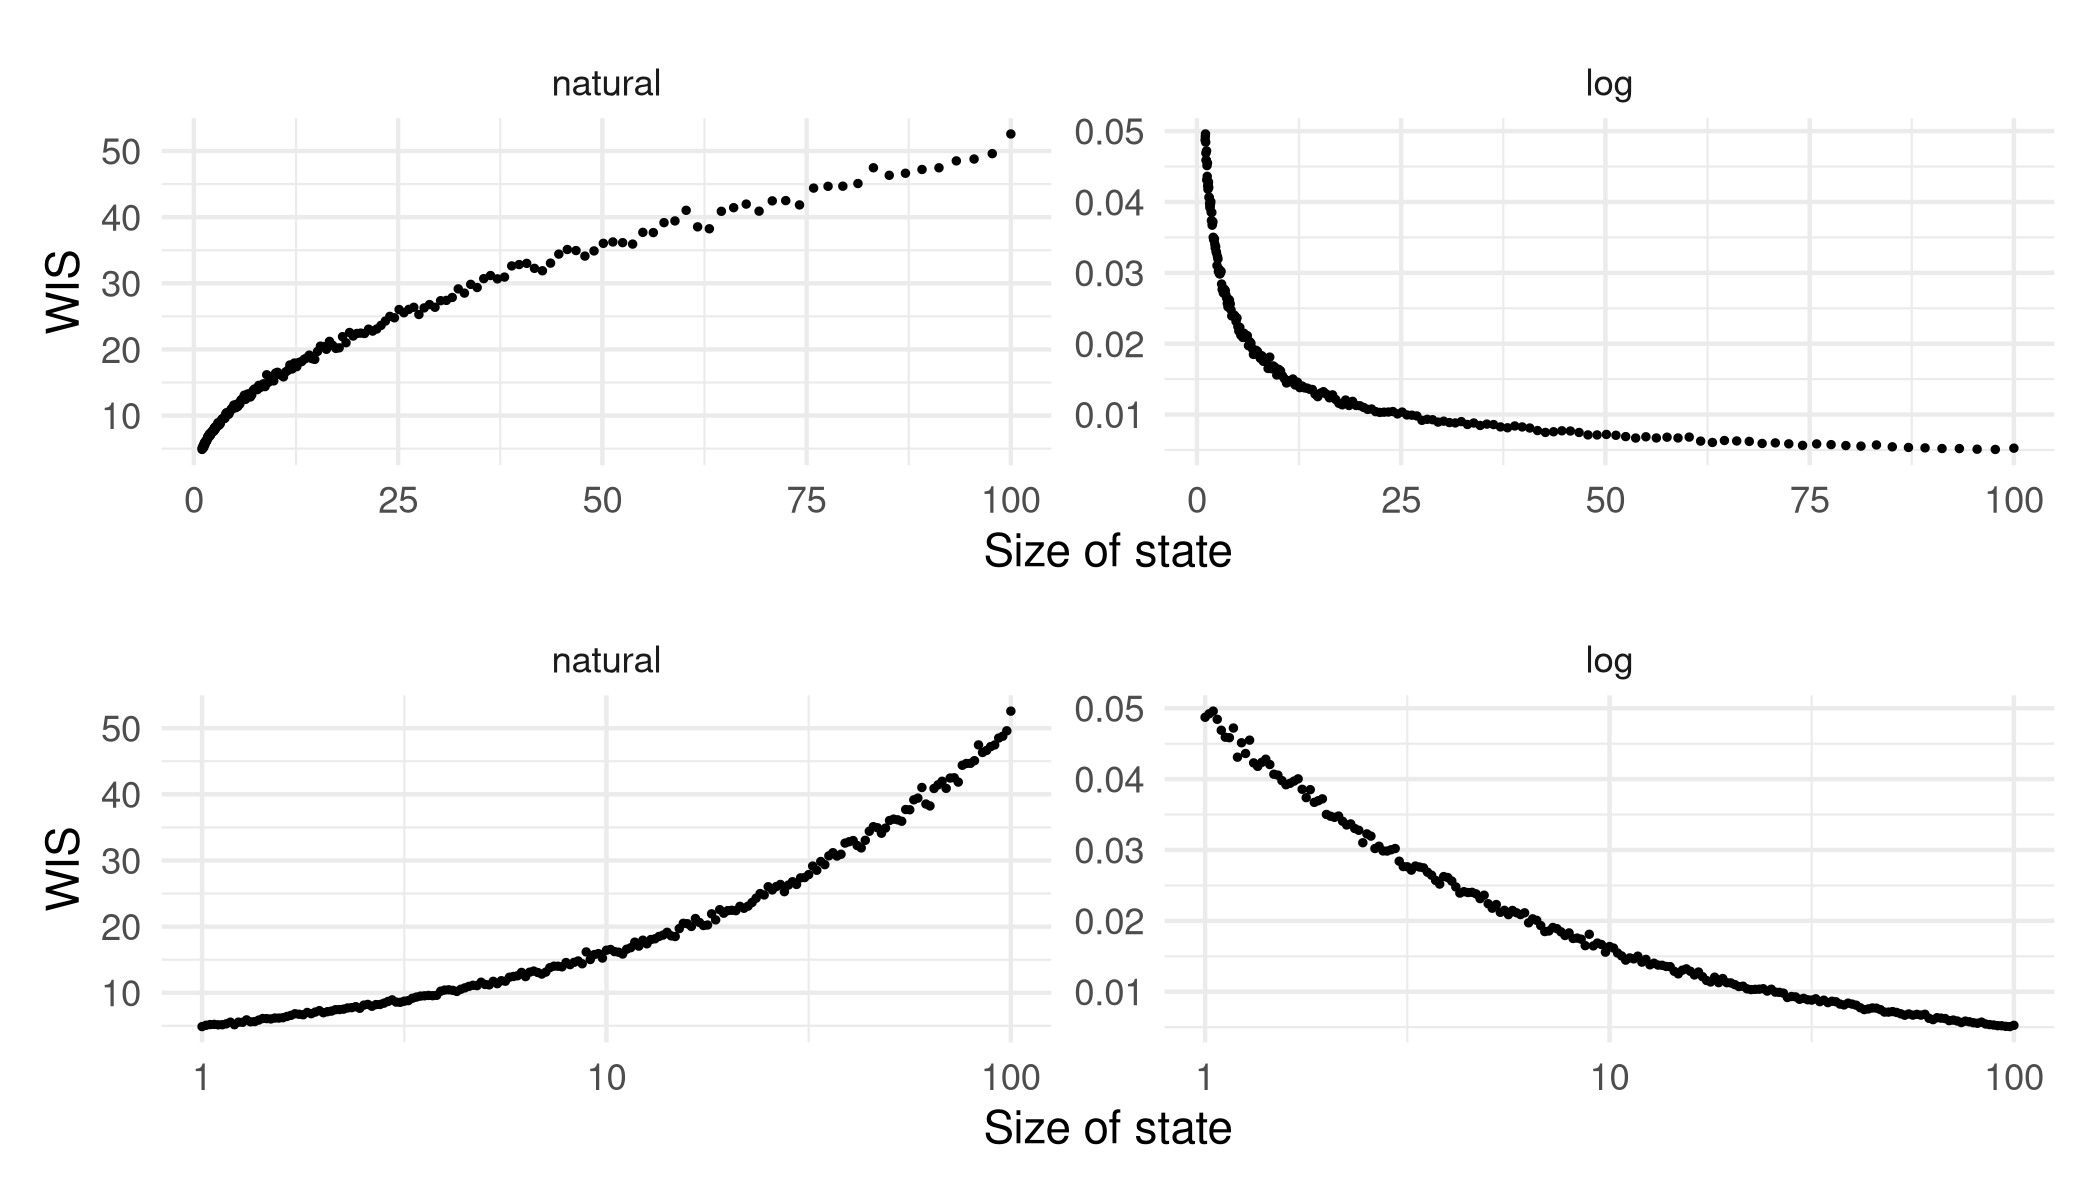
\includegraphics[width=0.9\textwidth]{output/figures/SIM-mean-sd-state-size.png}
    \caption{Simulation of the effect of population size with ideal forecasts of a negative-binomially-distributed variable. For each simulated state, we drew 1,000 observations from a negative binomial distribution with $\mu = 100 \cdot \text{state size}$ and with values of $\theta$ equal to 0.1, 1, and 1 billion. The variance of the negative binomial is given as $\sigma^2 = \mu + \mu^2 / \theta$, meaning that for large theta the negative binomial distribution is equal to the poisson distribution. For these simulated values we computed the WIS for an ideal forecast (i.e. the predictive distribution was negative binomial with $\mu$ and $\theta$ equal to the true $\mu$ and $\theta$ for every state). Left: Mean WIS depending on state size, right: Mean WIS depending on state sizes when scored on a log scale. Plots for the standard deviation, rather than the mean of WIS values look are given in Figure \ref{fig:SIM-wis-state-size-sd} in the SI.}. 
    \label{fig:SIM-wis-state-size-mean}
\end{figure}


Conveniently, the decomposition of the WIS into dispersion, overprediction and underprediction is preserved. The interpretation of the components has now changed in that they now (approximately) represent uncertainty, over-prediction, and under-prediction with the growth rate and so are independent of current incidence. 



%Score different things from the European / US Forecast Hub and plot the relationship between mean and variance. Plot log-scale scores for different things and see which of these influence average scores most \\
% What happens to the decomposition of the WIS if we log? 


%COMPARISON TO SCORING THE ACTUAL GROWTH RATE - just harder to do and achieves the same thing? No objections if someone wants to? Might actually be better if there are negative values involved? 

%What about other things like scoring the square root of the forecast?


%\begin{itemize}
%    \item discuss how equations change for CRPS
%    \item Optional: Discussion of parallels to point forecasts and the point that you're still incentivised to report the median\\
%    \item discuss that even if both scoring rules are proper, they still penalise different things %differently. How does that change incentives for the forecaster? 
%\end{itemize}


\paragraph{Toy example: simulate an epidemic and apply 3 different models} Compare scores for these three models on the natural scale and the log scale


\section{Empirical example: the European Forecast Hub}

\paragraph{Introduction to the Forecast Hub} As an empirical example for evaluating forecasts on the natural and on the log scale we use forecasts from the European Forecast Hub \citep{europeancovid-19forecasthubEuropeanCovid19Forecast2021}. Every week the European Forecast Hub collates and aggregates forecasts for different COVID-19 related targets from teams around the world. Forecasts are made one to four weeks ahead into the future and follow a quantile-based format with a set of 22 quantiles plus the median ($0.01, 0.025, 0.05, ..., 0.5, ... 0.95, 0.975, 0.99$). The forecasts for the purpose of this illustrations are two-week-ahead forecasts made between XXX and XXX for reported cases and deaths from COVID-19 in XXX countries. 

\paragraph{Describing features of the data}
Across all time points and locations, the mean number of cases (deaths) observed was 22811 (368) with an overall standard deviation of 47135 (831). The number of observed value does not only differ by forecast target, but also shows considerable heterogeneity by location (see Figure \ref{fig:HUB-mean-locations}. Across the different locations, the variance in observed values is roughly equal to the square of the mean, suggesting that, for a given location, both cases and deaths are not poisson-distributed, but rather exhibit over-dispersion. 
MAYBE FIT A NEGATIVE BINOMIAL TO THESE OBSERVATIONS

\begin{figure}[h!]
    \centering
    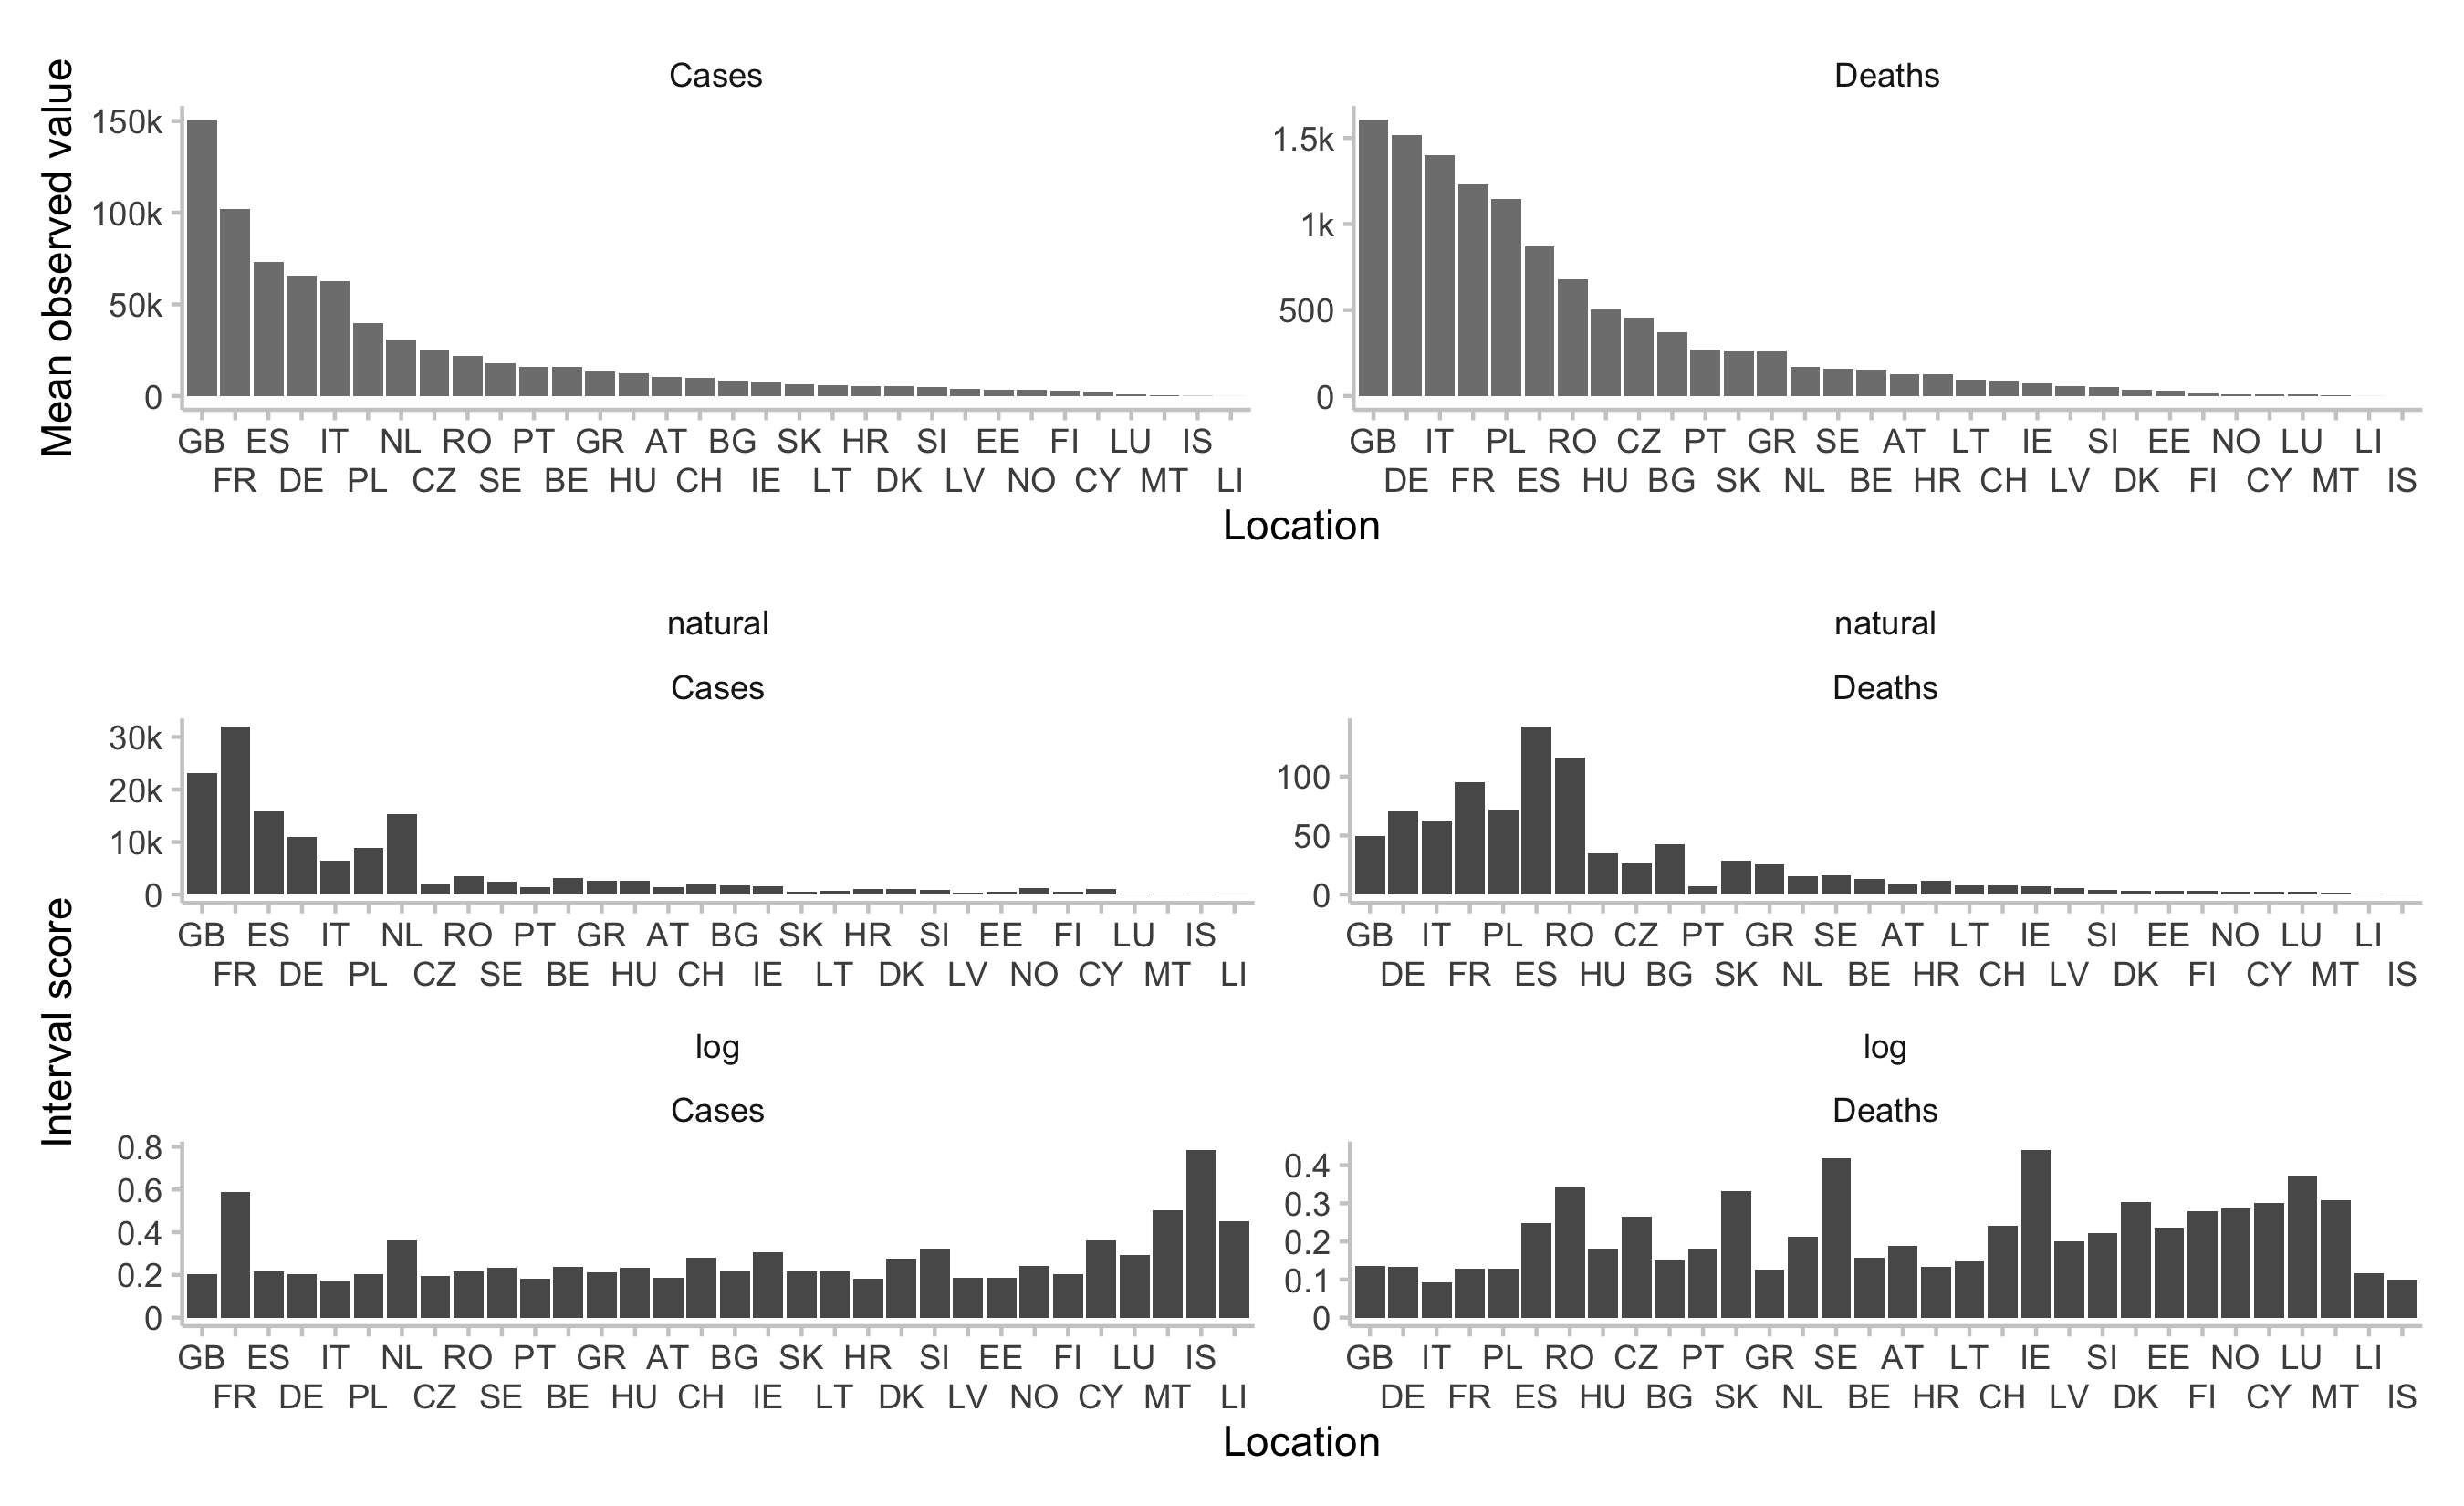
\includegraphics[width=0.9\textwidth]{output/figures/HUB-mean-obs-location.png}
    \caption{CAPTION}
    \label{fig:HUB-mean-locations}
\end{figure}

\paragraph{Features of the scores}
Across all time points and locations, the mean number weighted interval score on the natural scale for cases (deaths) was 8855 (59.3) with an overall standard deviation of 51274 (156). On the log scale, scores were much closer to each other (see Figure \ref{fig:HUB-average-scores}), with a mean WIS for cases (deaths) of 0.507 (0.362) with an overall standard deviation of 0.745 (0.407). 
% NEED A TABLE WITH SCORES for the Appendix
On the natural scale, scores vary by several orders of magnitudes across locations (see \ref{fig:HUB-scores-location}), whereas variation across locations is much smaller for scores on the log scale and wis values are more evenly distributed. The ordering of scores across locations is not preserved when going from the natural to the log scale. 
% Rather, there seems to be a slight inverse relationship that locations which previously had low scores now tend to receive higher scores. 
The correlation between scores on the log and natural scale for different locations is XX for cases and XX for deaths. 
%THERE SEEMS TO BE A TENDENCY FOR SMALLER 

\begin{figure}[h!]
    \centering
    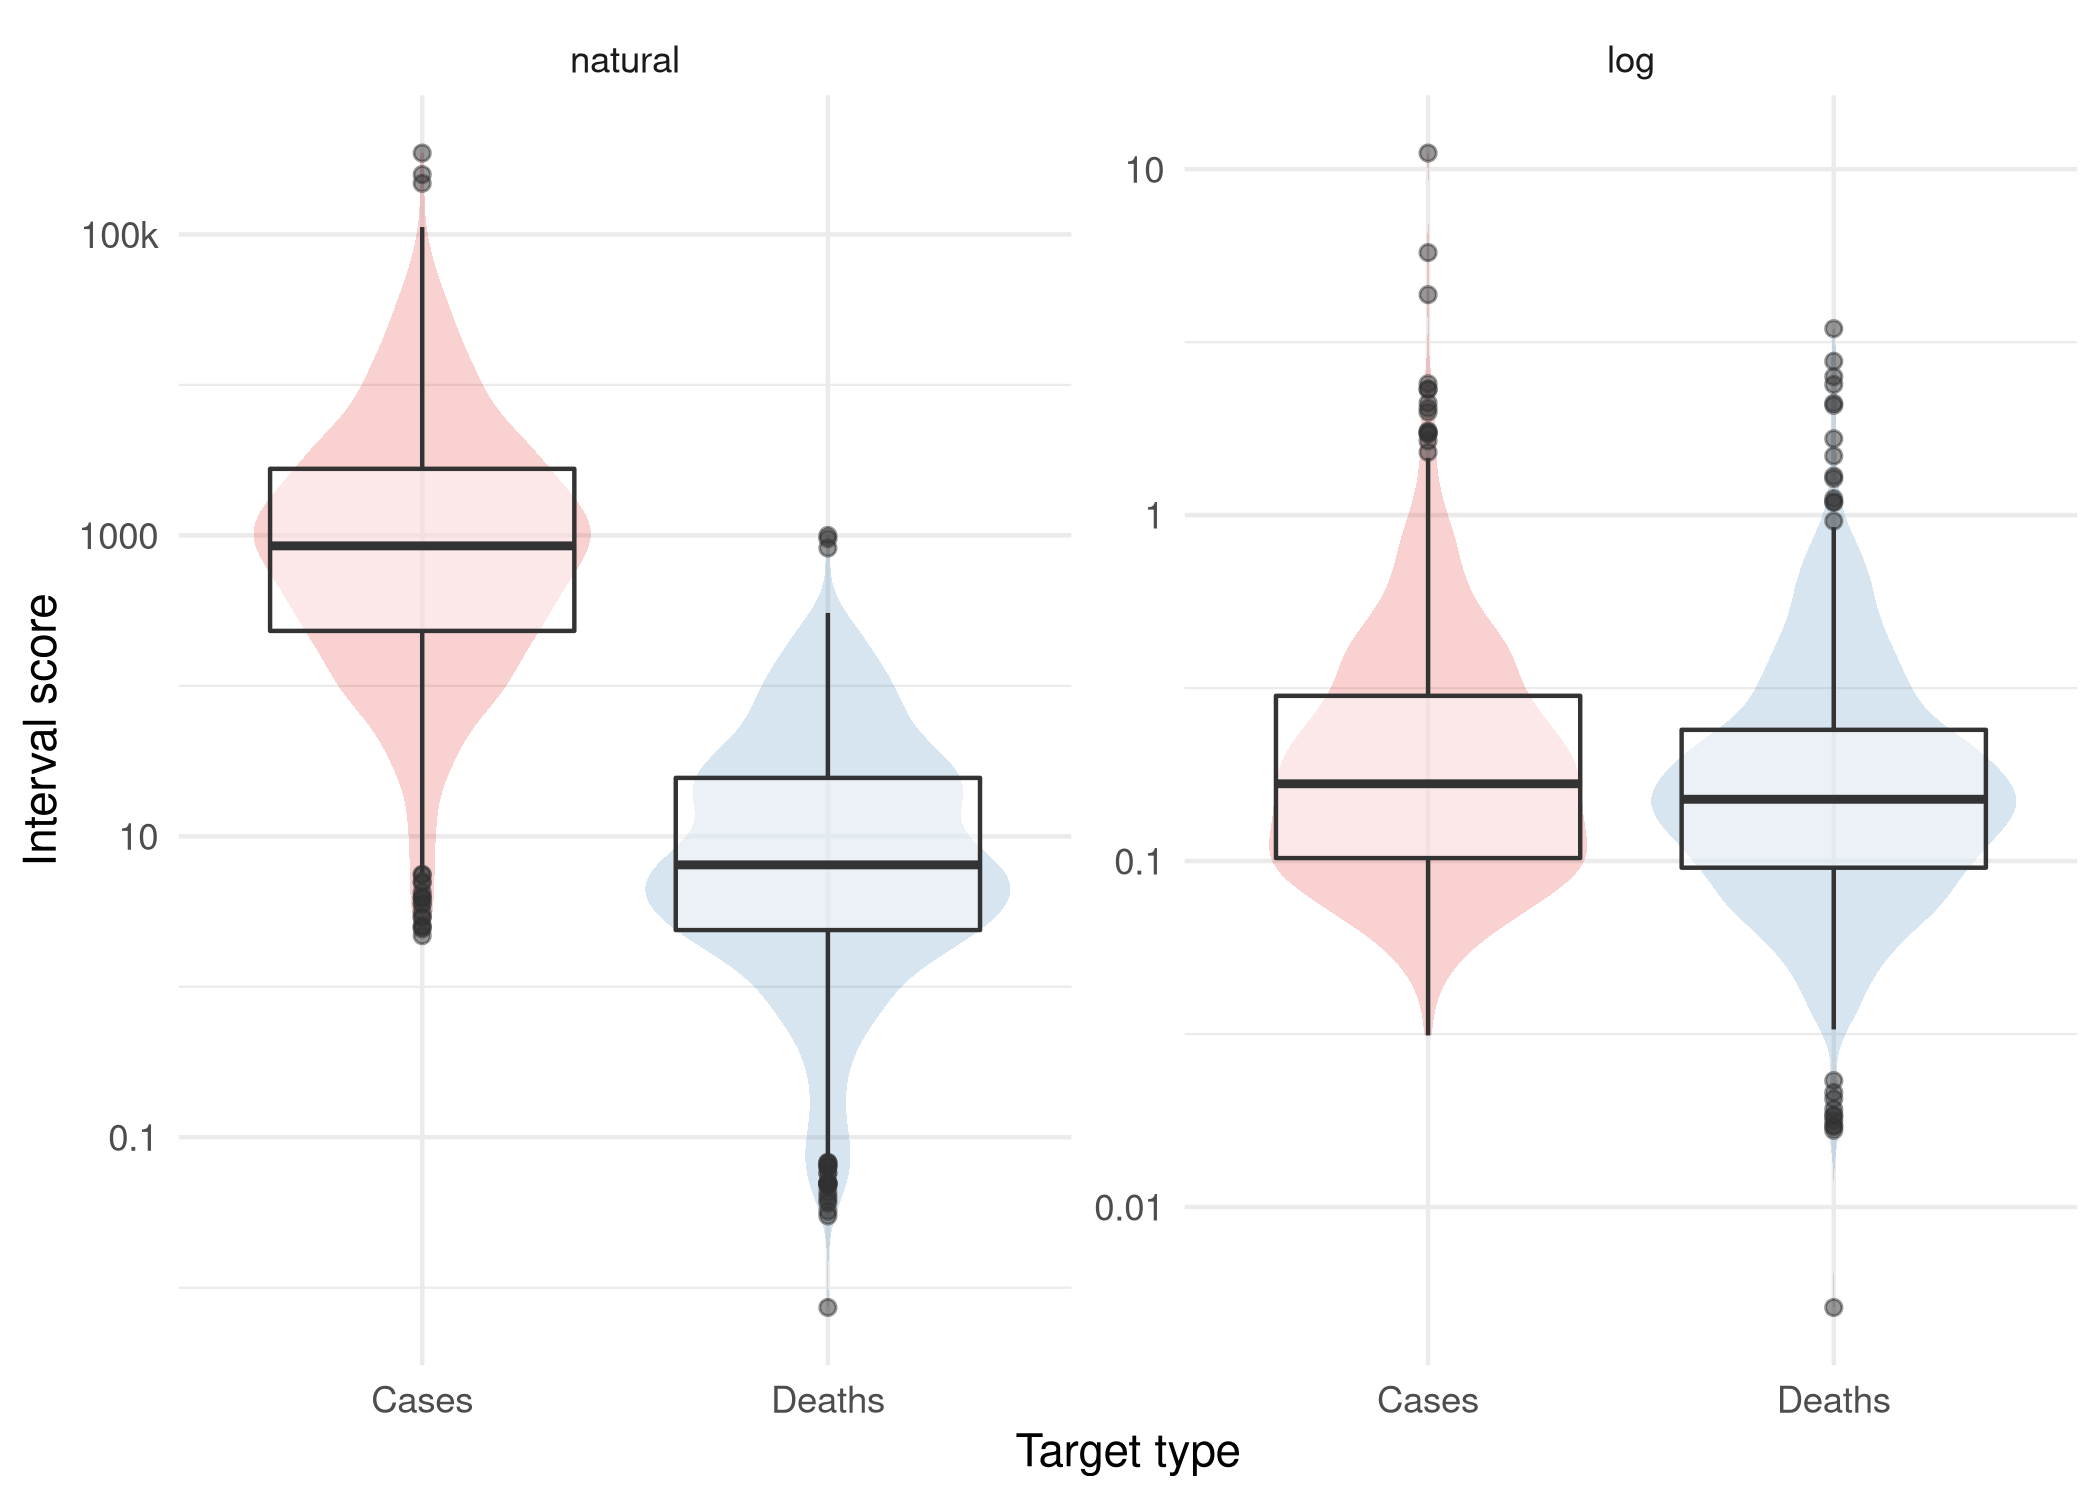
\includegraphics[width=0.9\textwidth]{output/figures/HUB-average-scores.png}
    \caption{Distribution of interval scores for two week ahead forecasts of COVID-19 cases and deaths evaluated on the natural scale (left) and on the log scale (right). }
    \label{fig:HUB-average-scores}
\end{figure}

\begin{figure}[h!]
    \centering
    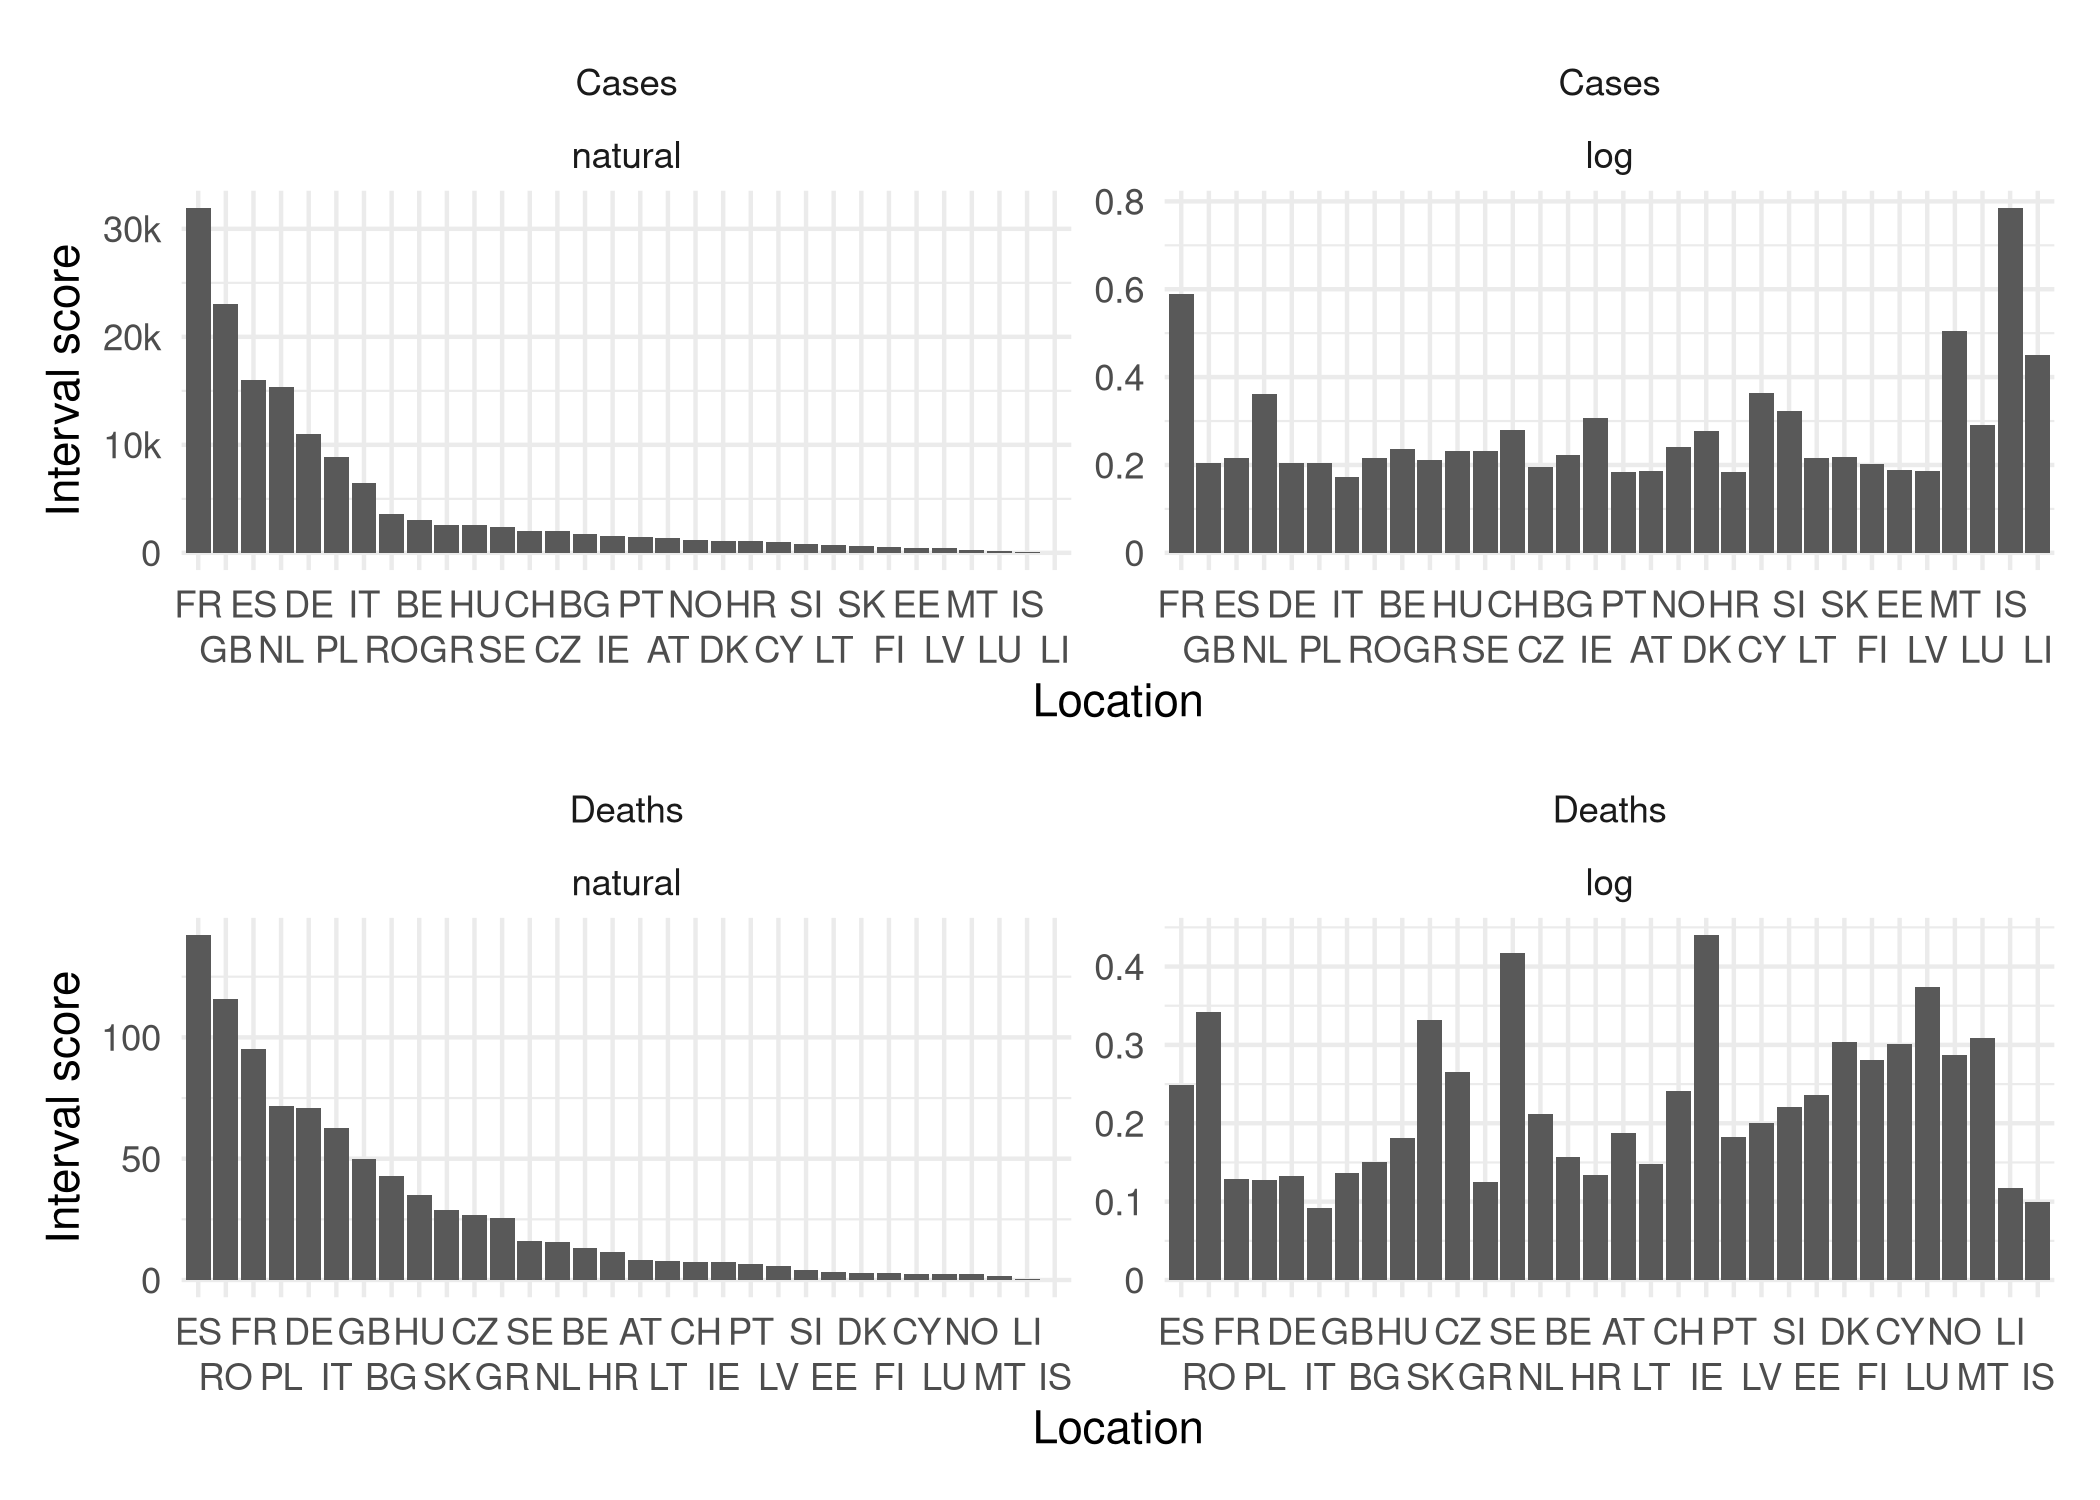
\includegraphics[width=0.9\textwidth]{output/figures/HUB-scores-locations.png}
    \caption{Weighted interval scores across different locations for two week ahead forecasts of COVID-19 cases and deaths evaluated on the natural scale (left) and on the log scale (right). }
    \label{fig:HUB-scores-location}
\end{figure}
% Could also sort this figure according to population size?
%Make multi panel Figure with Figure 2 and sort according to mean outcome

When evaluated on the natural scale, there is  strong relationship between the mean of the weighted interval score and the total number of observed cases (correlation: 0.913) or deaths (cor: 0.849) in a location (see Figure \ref{fig:HUB-mean-scores-total-loglog} and Figure \ref{fig:HUB-mean-scores-total} in the SI). The relationship is less pronounced for scores on the log scale (cor: -0.019 for cases, -0.395 for deaths) and negative, meaning that locations with fewer observed cases or deaths tend to receive higher scores. 

\begin{figure}[h!]
    \centering
    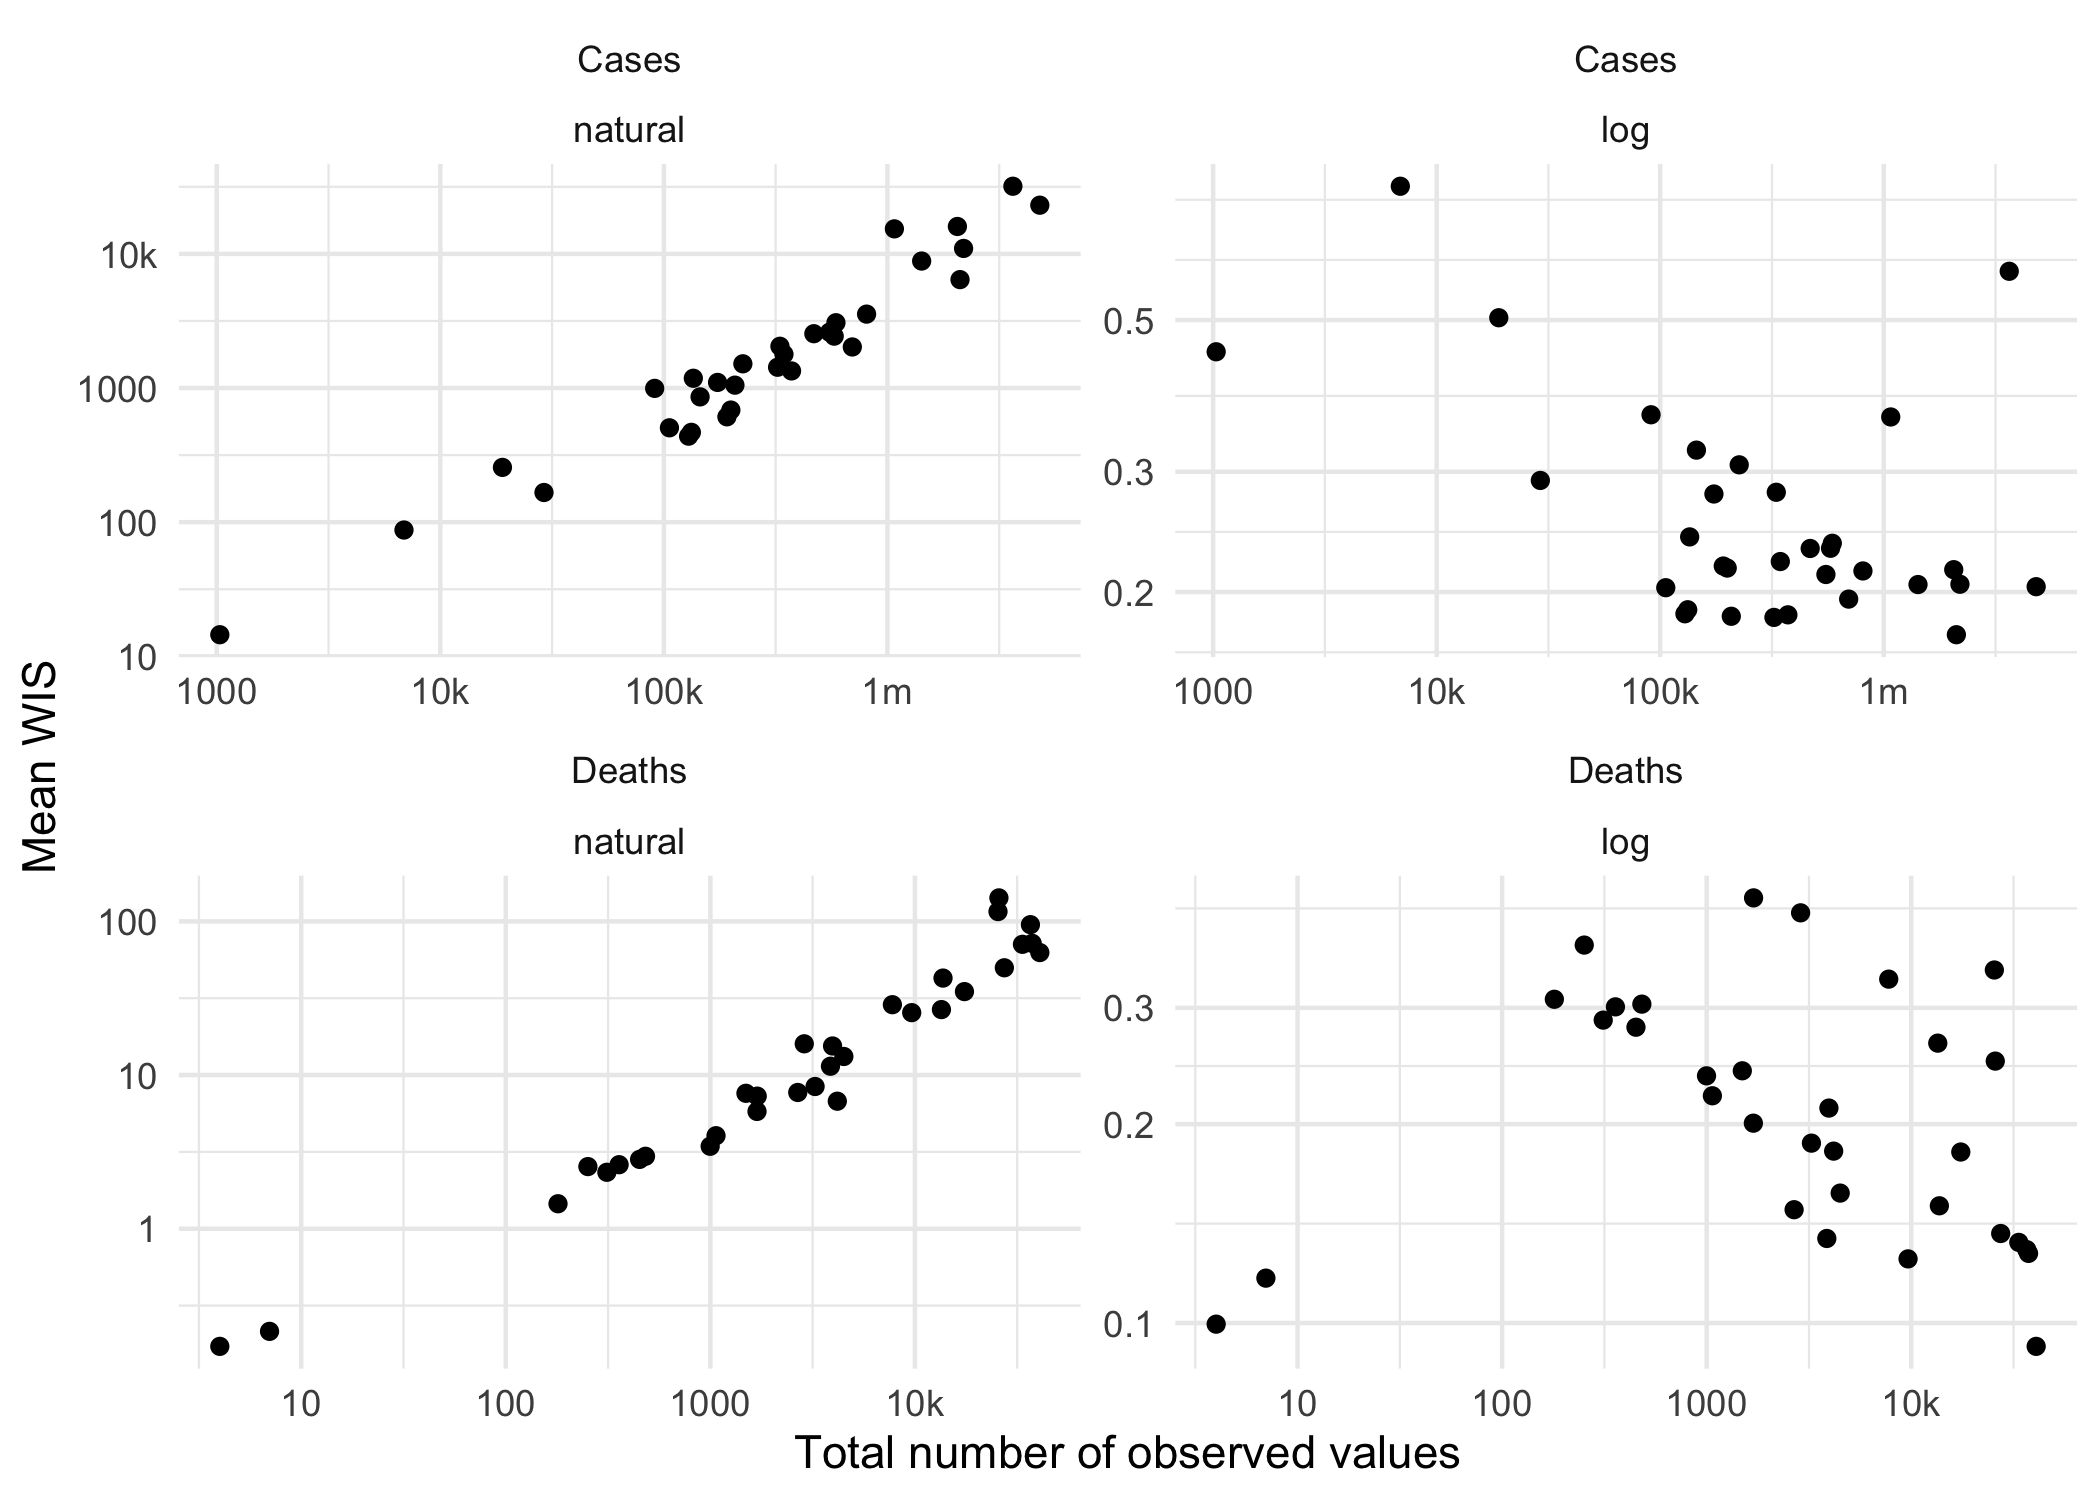
\includegraphics[width=0.9\textwidth]{output/figures/HUB-mean-scores-vs-total-log-log.png}
    \caption{Plot with Weighted interval scores against the mean number of observed cases or deaths.}
    \label{fig:HUB-mean-scores-total-loglog}
\end{figure}

Both on the natural scale as well as on the log scale, scores increase considerably with increasing forecast horizon (see Figure \ref{fig:HUB-scores-horizon}). The increase is more pronounced for cases than for deaths and arguably represents an increase in the relative difficulty to forecast values further into the future. A similar increase both on the natural and the log scale indicates that we are able to observe the increase in difficulty regardless of how we evaluate the scores. 

\begin{figure}[h!]
    \centering
    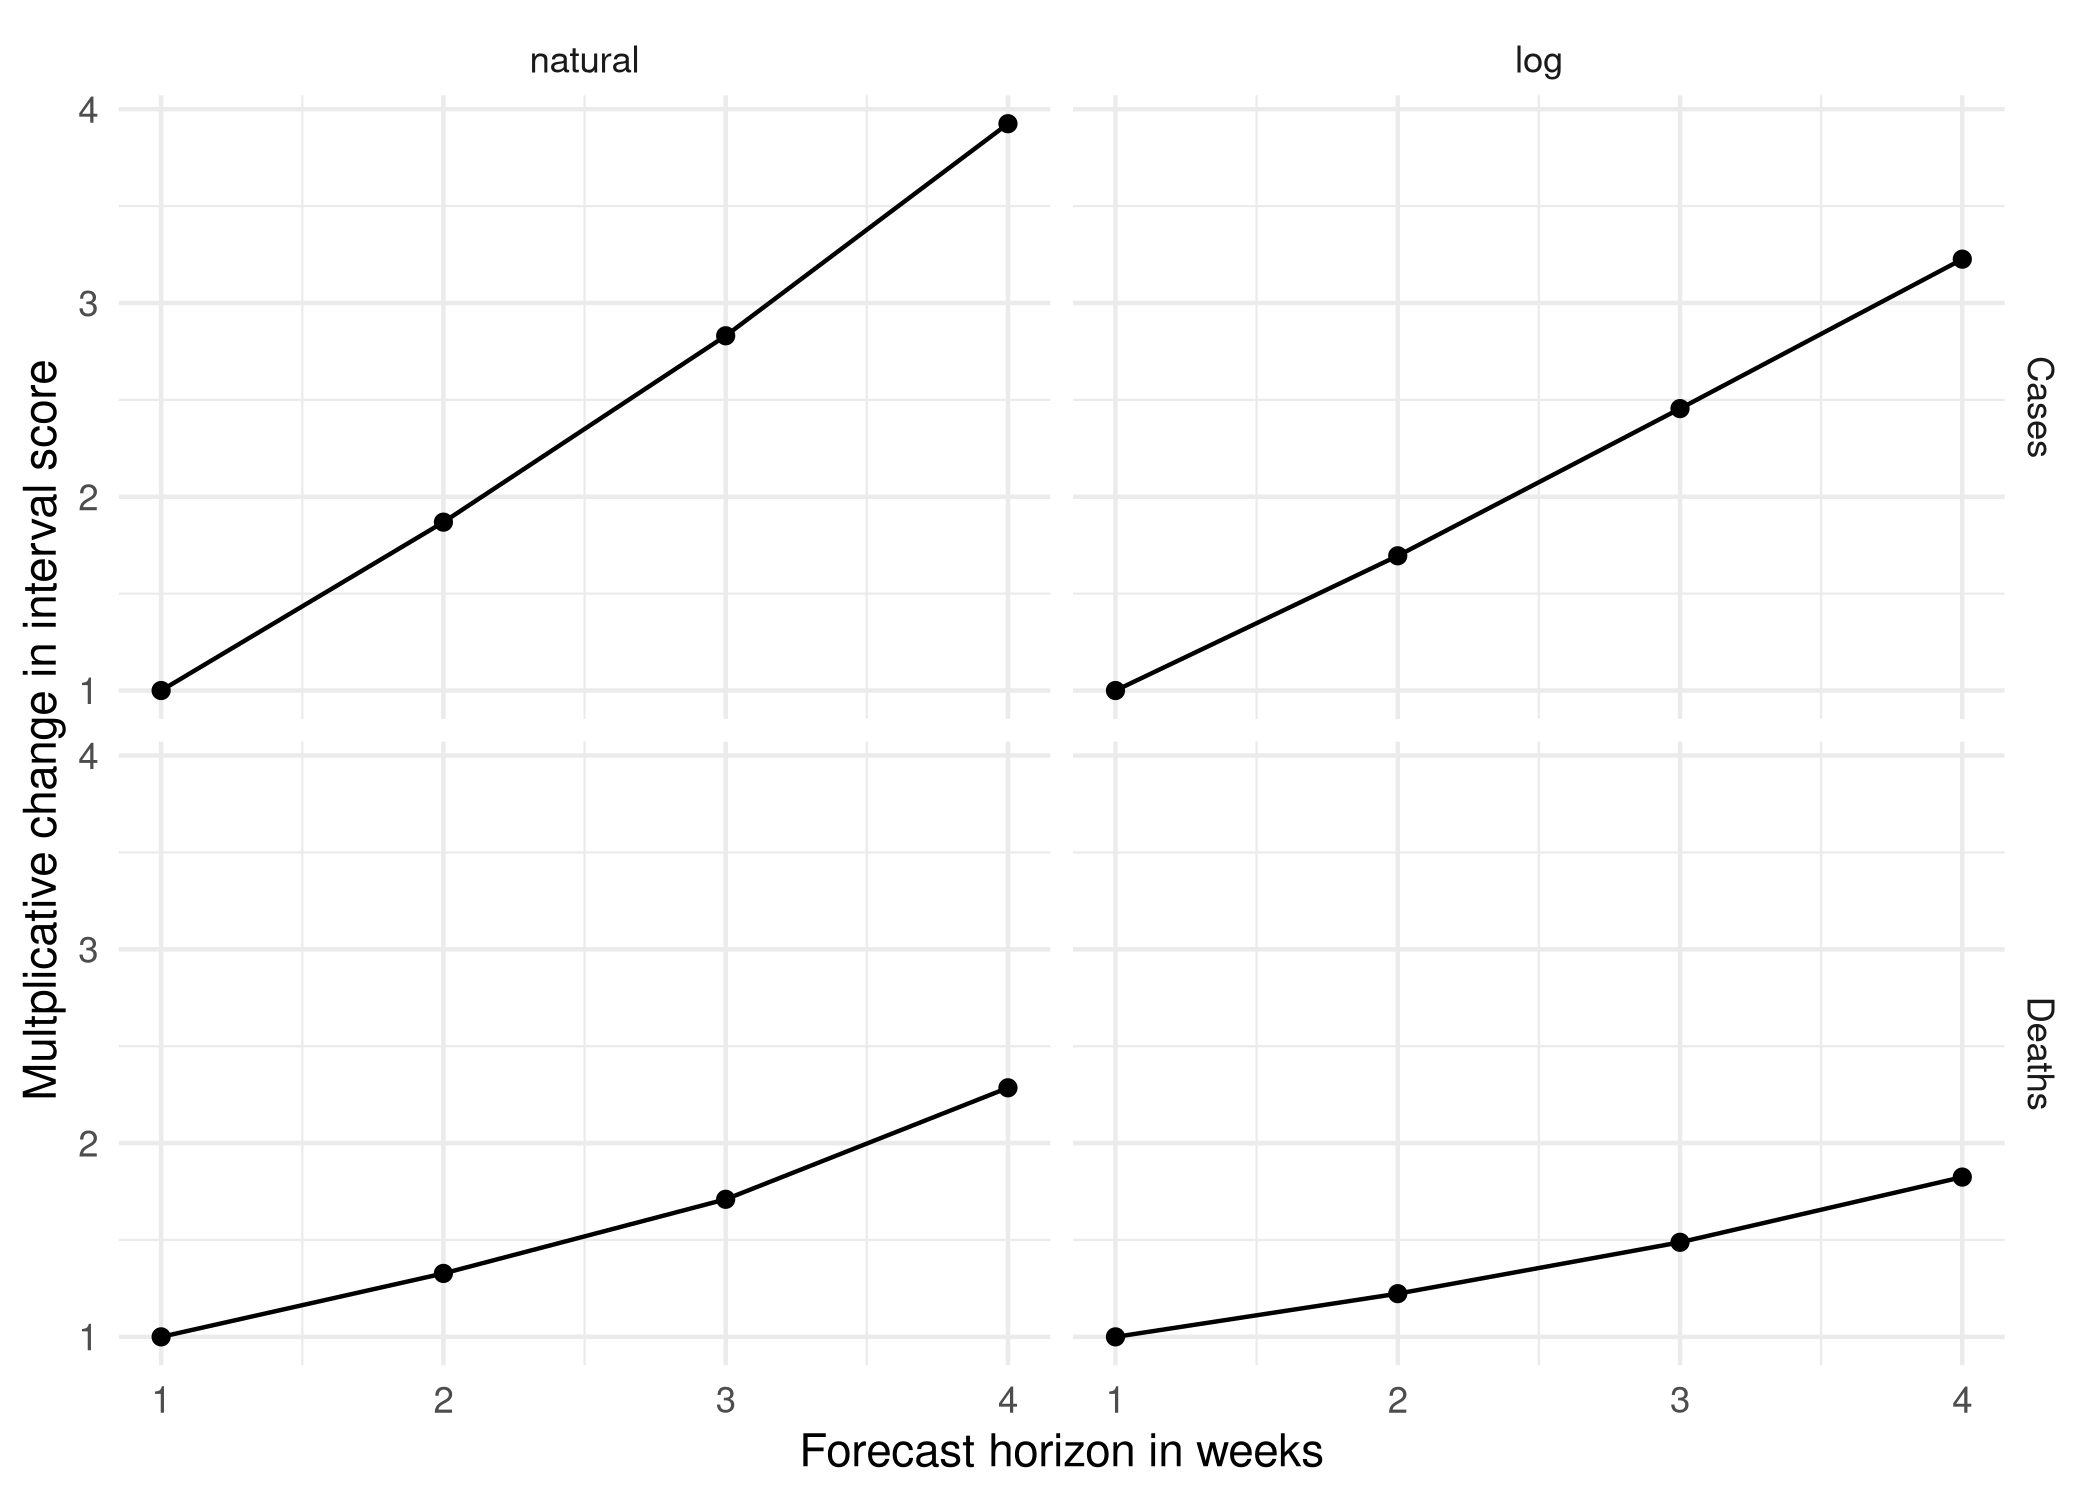
\includegraphics[width=0.9\textwidth]{output/figures/HUB-scores-over-horizon.png}
    \caption{Weighted interval scores across forecast horizons}
    \label{fig:HUB-scores-horizon}
\end{figure}



% \section{Other ideas}
% \begin{itemize}
%     \item Compare different predictive distributions and the score as a function of an outcome.
%     \item ...
% \end{itemize}




\section{Discussion}

\paragraph{summary of what we did}

\paragraph{context, implications, limitations}

SOME DIFFERENCES BETWEEN SCORES ARE MEANINGFUL. E.G. WE WOULDN'T WANT SCORES FOR CASES AND DEATHS TO BE COMPLETELY EQUAL, BECAUSE DEATHS ARE LIKELY EASIER TO FORECAST

\paragraph{outlook, future work}


 




\newpage

\appendix
\section{Supplementary information}


\subsection{Additional information on the WIS} \label{wis}
\paragraph{WIS}

WIS values are always larger or equal than zero and lower values imply better performance. The WIS can be decomposed into a dispersion component and penalties for over- and under-prediction. For a single prediction interval, the interval score is computed as 
\begin{align}
 IS_\alpha(F,y) &= (u-l) + \frac{2}{\alpha} \cdot (l-y) \cdot 1(y \leq l) + \frac{2}{\alpha} \cdot (y-u) \cdot 1(y \geq u) \\
 &= \text{dispersion} + \text{underprediction} + \text{overprediction},    
\end{align}

where $1()$ is the indicator function, $y$ is the observed value, and $l$ and $u$ are the $\frac{\alpha}{2}$ and $1 - \frac{\alpha}{2}$ quantiles of the predictive distribution $F$, i.e. the lower and upper bound of a single central prediction interval. For a single forecast interval, the interval score is the width of the prediction interval, if it covers the observed value, and the absolute error between the forecast and the lower (or upper, respectively) interval boundary. For a set of $K$ prediction intervals and the median $m$, the WIS is computed as a weighted sum, 
\begin{equation}
\text{WIS} = \frac{1}{K + 0.5} \cdot \left(w_0 \cdot |y - m| + \sum_{k = 1}^{K} w_k \cdot IS_{\alpha}(F, y)\right),    
\end{equation} 
where $w_k$ is a weight for every interval. Usually, $w_k = \frac{\alpha_k}{2}$ and $w_0 = 0.5$. 


The WIS is closely related to the continuous ranked probability score (CRPS) [Cite Gneiting 2007], which itself can be understood as a generalisation of the absolute error to probabilistic forecasts. For an increasing set of equally-spaced prediction intervals the WIS converges to the CRPS and shares many of its properties. More information on the CRPS is provided in section \ref{crps} in the SI. 

\subsection{Additional information on the CRPS} \label{crps}

The CRPS measures the 'distance' of the predictive distribution to the observed data-generating distribution as 

\begin{equation}
    \text{CRPS}(F, y) = \int_{-\infty}^\infty \left( F(x) - 1(x \geq y) \right)^2 dx,
\end{equation}

where y is the true observed value and F the CDF of predictive distribution. Often the following alternative representation is used
\begin{equation}
    \text{CRPS}(F, y) = \frac{1}{2} \mathbb{E}_{F} |X - X'| - \mathbb{E}_P |X - y|,
\end{equation}
  
where $X$ and $X'$ are independent realisations from the predictive distributions $F$ with finite first moment and $y$ is the true value. In this representation we can simply replace $X$ and $X'$ by samples sum over all possible combinations to obtain the CRPS.  





\subsection{Scoring the growth rate directly}
By dividing every observed value and every forecast by the last observed value prior to evaluation, we replace forecasting $y_{t+1}$ with forecasting  $y_{t+1} / y_t = 1 + g_{t, t+1}$. Just as we were previously penalised an additive error with respect the absolute value, we are now penalising an absolute error with respect to the growth rate. 

We can illustrate what's happening by thinking of an analogous point prediction $\hat{g_{t, t+1}}$ for the growth rate. We could then write
\begin{equation}
    1 + g_{t, t+1} = 1 + \hat{g}_{t, t+1} + \varepsilon^*_{t+1}. 
\end{equation}
%
The WIS and CRPS would evaluate the forecast based on the error $\varepsilon^*_{t+1}$. This translates to an absolute error on the actual forecast target that is multiplicatively connected to the last observed value: 
\begin{align}
    y_{t+1} &= (1 + \hat{g}_{t, t+1} + \varepsilon^*_{t+1}) \cdot y_t \\
            &= (1 + \hat{g}_{t, t+1}) \cdot y_t + \varepsilon^*_{t+1} \cdot y_t \\
            &= \hat{y}_{t+1} + \varepsilon^*_{t+1} \cdot y_t.
\end{align}

One disadvantage of this is that we can't really do anything when an observation is zero. 
%is this helpful?%
%Maybe add some math on how we actually transform the distribution. E.g. divide every quantile or sample by the last observed value, divide the distribution?%


\subsection{Changes in the WIS for forecasts on the log scale} \label{wis-log-derivation}

This connection with the underlying epidemic growth rate is an attractive property in and of itself as it is the conceptual target many forecasters and forecast consumers make use of. 

When we score a forecast for $y_{t+1}$ on the log scale, the interval score for a single prediction interval changes as follows
%
\begin{align}
    \text{IS}_\alpha(\log F, \log y) = &(\log u - \log l) \\ 
    &+ \frac{2}{\alpha} \cdot (\log l - \log y) \cdot 1(\log y \leq \log l) \\
    &+ \frac{2}{\alpha} \cdot (\log y - \log u) \cdot 1(\log y \geq \log u).
\end{align}
%
Note that the values of the indicator functions stay the same as the logarithm is a monotonic transformation and the inequality is preserved. 
On the natural scale, $u$, $l$ are the lower and upper bounds of a central prediction interval for a forecast of $y_{t+1} = (1 + g_{t, t+1}) \cdot y_t$. 
We can rewrite these as 
\begin{equation}
   l = l^* \cdot y_t 
   \;\; \text{and} \;\; 
   u = u^* \cdot y_t,  
\end{equation}
where $u^*$ and $l^*$ are the lower and upper bounds of a prediction interval for $(1 + g_{t, t+1})$. Consequently, 
\begin{equation}
  \log l = \log l^* + \log y_t
  \;\; \text{and} \;\;
  \log u = \log u^* + \log y_t. 
\end{equation}
%
We can then rewrite the score for a forecast of $\log y_{t+1} = \log (1 + g_{t,t+1}) + \log y_t$ as
%
\begin{equation}
\begin{aligned}
IS_\alpha&(\log F_{t+1}, \log y_{t+a}) = \\
&((\log u^* + \log y_t) - (\log l^* + \log y_t)) \\
&+ \frac{2}{\alpha} \cdot ((\log l^* + \log y_t) - (\log (1 + g_{t, t+1}) + \log y_t)) 
     \cdot 1((\log (1 + g_{t, t+1}) + \log y_t) \leq (\log l^* + \log y_t) \\
&+ \frac{2}{\alpha} \cdot ((\log (1 + g_{t, t+1}) + \log y_t) - (\log u^* + \log y_t)) 
      \cdot 1((\log (1 + g_{t, t+1}) + \log y_t) \geq (\log u^* + \log y_t),
\end{aligned}
\end{equation}
%
which simplifies to 
%
\begin{equation}
\begin{aligned}
\label{eqn:is-log}
\text{IS}_\alpha(\log F_{t+1}, \log y_{t+a}) = &(\log u^* - \log l^*) \\
&+ \frac{2}{\alpha} \cdot (\log l^* - \log (1 + g_{t, t+1}) 
     \cdot 1(\log (1 + g_{t, t+1}) \leq \log l^*) \\
&+ \frac{2}{\alpha} \cdot (\log (1 + g_{t, t+1}) - \log u^*) 
      \cdot 1(\log (1 + g_{t, t+1}) \geq \log u^*).
\end{aligned}
\end{equation}

The left-hand side of equation \ref{eqn:is-log} was left unchanged. From the right-hand side we can see that for a single prediction interval, scoring the log of a forecast ($\log F_{t+1}$) against the log observed value ($\log y_{t+1}$) is exactly equivalent to evaluating a forecast for $\log (1 + g_{t, t+1})$. With $\log (1 + g_{t, t+1} \approx g_{t, t+1}$, this is approximately a forecast for the growth rate for small values of $g_{t, t+1}$. 


\subsection{Additional figures}




\begin{figure}[h!]
    \centering
    
\includegraphics[width=0.9\textwidth]{output/placeholder-image.png}
    \caption{Illustration of the fact that taking the log of WIS or CRPS results in an improper score}
    \label{fig:log-improper}
\end{figure}


\begin{figure}[h!]
    \centering
    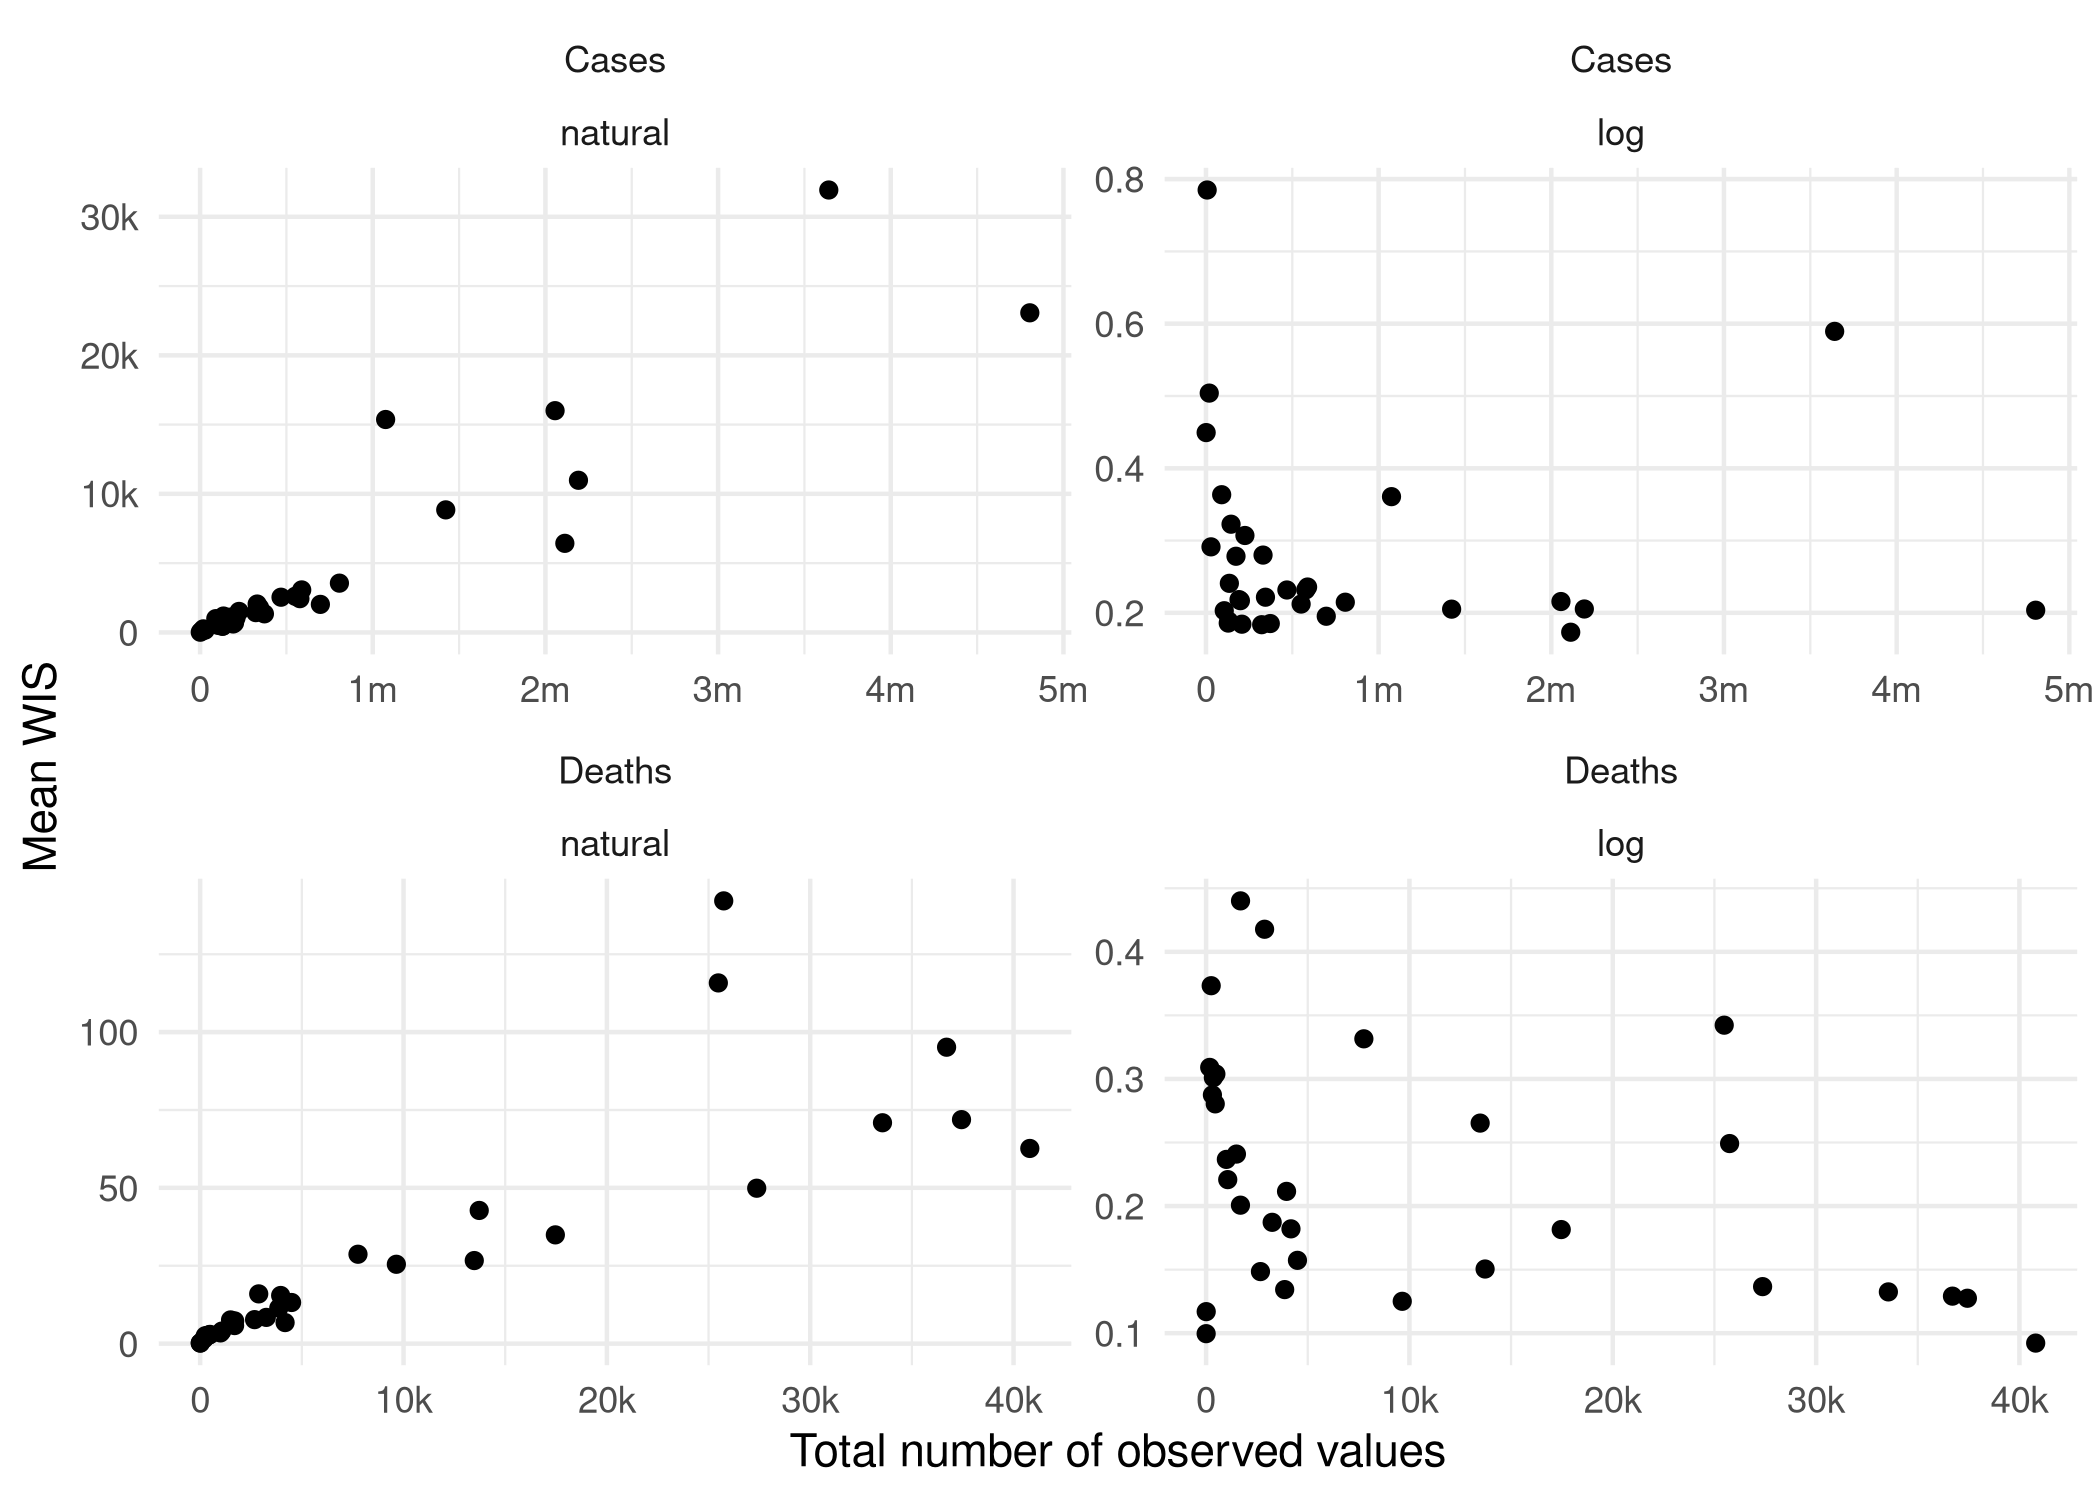
\includegraphics[width=0.9\textwidth]{output/figures/HUB-mean-scores-vs-total.png}
    \caption{Plot with Weighted interval scores against the mean number of observed cases or deaths.}
    \label{fig:HUB-mean-scores-total}
\end{figure}

\begin{figure}[h!]
    \centering
    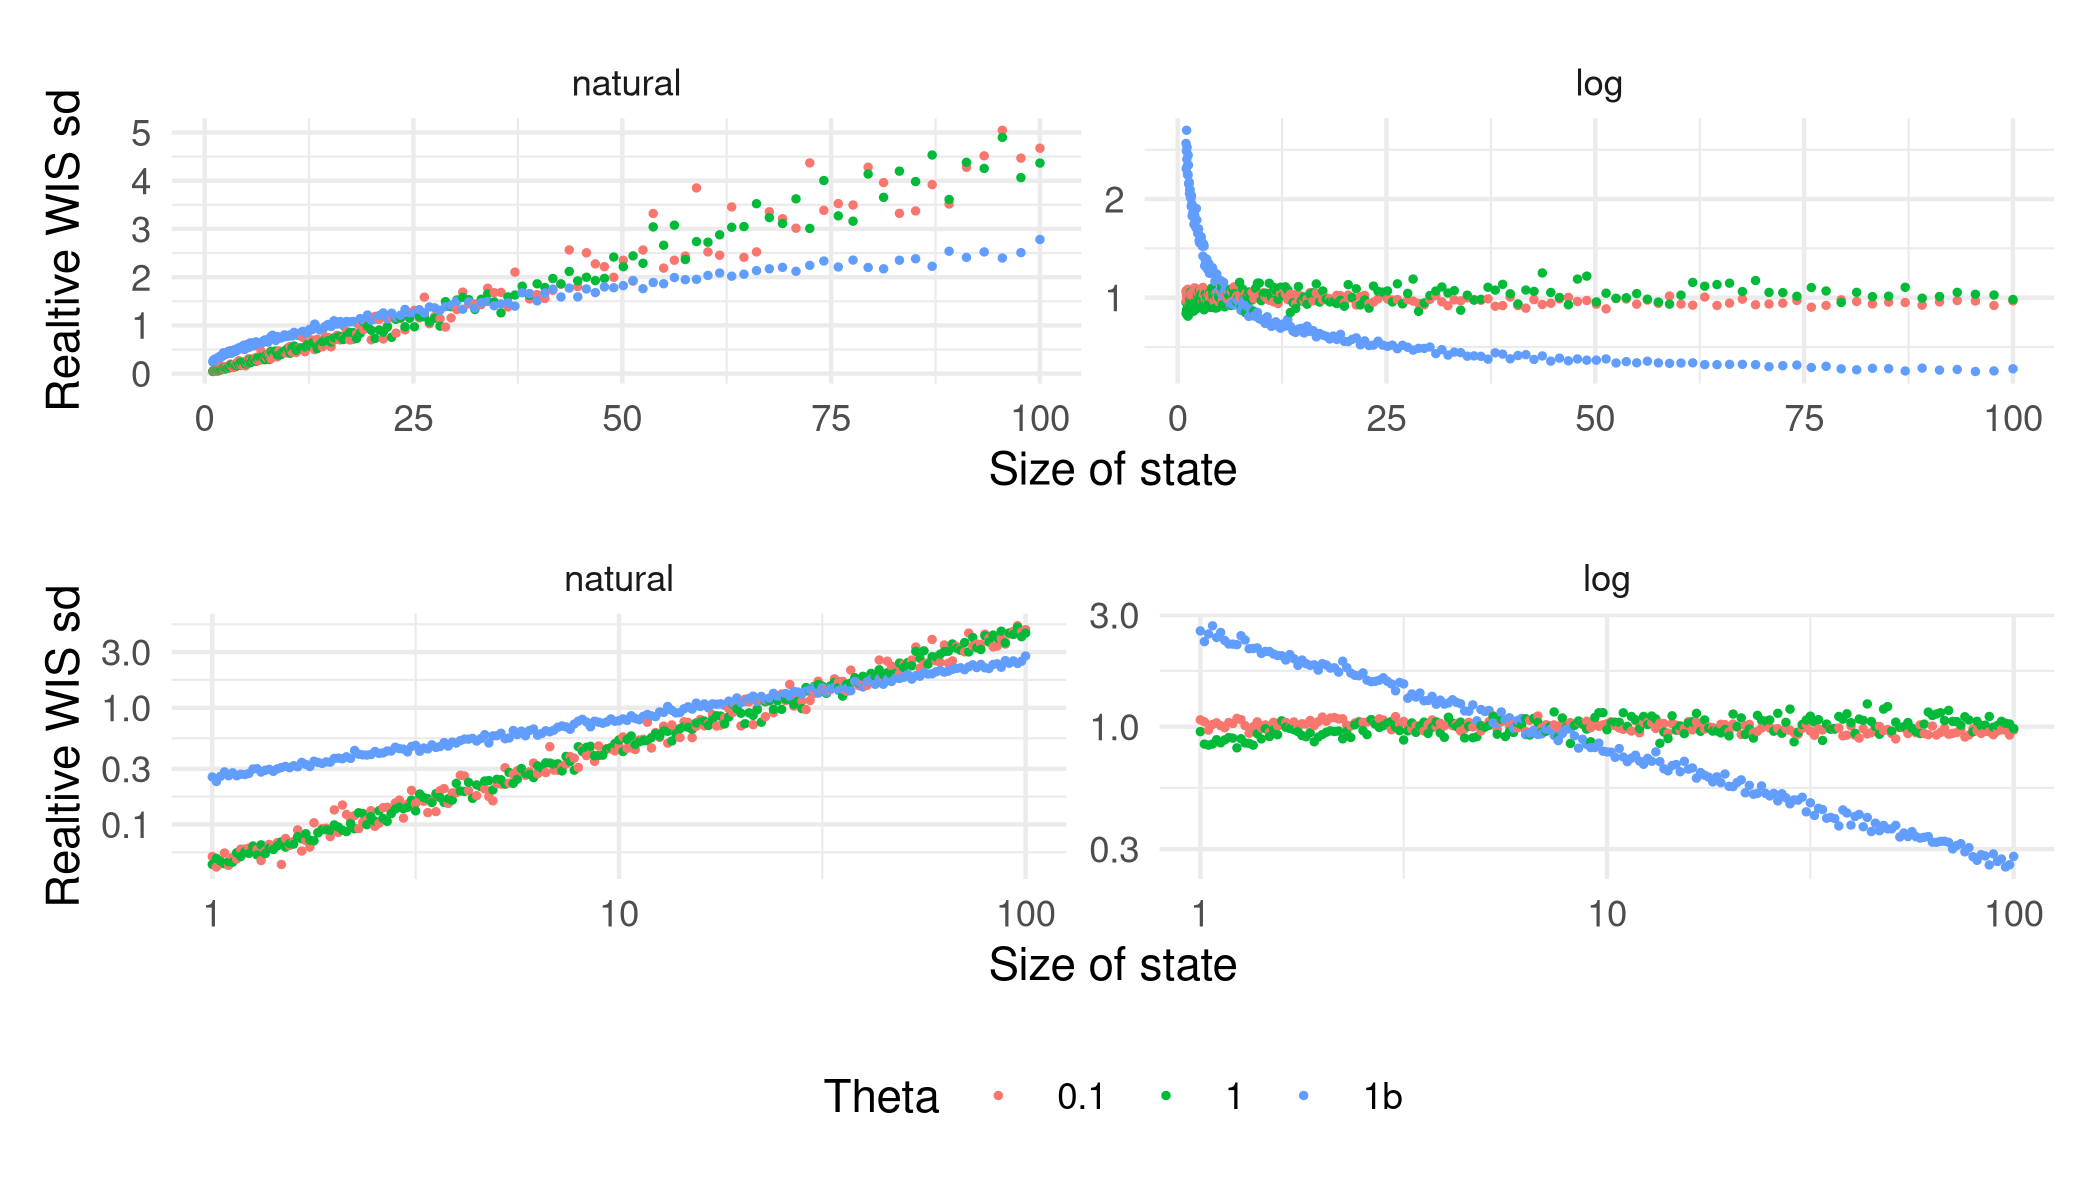
\includegraphics[width=0.9\textwidth]{output/figures/SIM-sd-state-size.png}
    \caption{Simulation of the effect of population size with ideal forecasts of a negative-binomially-distributed variable. For each simulated state, we drew 1,000 observations from a negative binomial distribution with $\mu = 100 \cdot \text{state size}$ and with values of $\theta$ equal to 0.1, 1, and 1 billion. The variance of the negative binomial is given as $\sigma^2 = \mu + \mu^2 / \theta$, meaning that for large theta the negative binomial distribution is equal to the poisson distribution. For these simulated values we computed the WIS for an ideal forecast (i.e. the predictive distribution was negative binomial with $\mu$ and $\theta$ equal to the true $\mu$ and $\theta$ for every state). Left: Mean WIS depending on state size, right: Mean WIS depending on state sizes when scored on a log scale. Plots for the standard deviation, rather than the mean of WIS values look are given in Figure \ref{fig:SIM-wis-state-size-sd} in the SI.}. 
    \label{fig:SIM-wis-state-size-mean}
\end{figure}



\end{document}


%%%%%%%%%%%%%%%%%%%%%%%%%%%%%%%%%%%%%%%%%%%%%%%%%%%%%%%%%%%%%%%%%%%%%%%%%%%%
% Idea parking lot 
%%%%%%%%%%%%%%%%%%%%%%%%%%%%%%%%%%%%%%%%%%%%%%%%%%%%%%%%%%%%%%%%%%%%%%%%%%%%

% NOT SO CONVINCED ANYMORE THAT THIS WORKS. MY INTUITION IS IF YOU WANT THE GROWTH RATE YOU SHOULD ACTUALLY SCORE THE GROWTH RATE AND DIVIDE BY THE LAST OBSERVED VALUE. 
% 
% WELL MAYBE IT WORKS AFTER ALL AND IT WOULD BE THE EQUIVALENT OF LOGGING FIRST AND THEN SUBTRACTING THE LAST OBSERVED VALUE WAIT A MINUTE THAT'S A DIFFERENT TRANSFORMATION AND ALSO THAT's SCORING THE LOG GROWTH RATE. 
% 
% BUT THEN AGAIN I'M STILL CONFUSED, BECAUSE ANY RELATIVE ERROR ON A QUANTITY Y\_t+1 IS AUTOMATICALLY AN ABSOLUTE ERROR ON THE GROWTH RATE IF WE KNOW Y\_t. AH BUT YOU DON'T KNOW WHAT THE ABSOLUTE ERROR ON THE GROWTH RATE IS (E.G. FOR Y\_t+1 of 10 IF YOU DON'T SPECIFICALLY LOOK AT THE LAST VALUE. BUT WE ARE ASSUMING THAT THIS IS WHAT THE MODEL DOES WHEN IT MAKES A FORECAST INTERNALLY




% The WIS can be thought of as an approximation of the CRPS for forecasts where the predictive distribution is represented through a set of quantiles. The CRPS, and by extension the WIS, represents a generalisation of the absolute error to continuous distributions, meaning that forecasters are evaluated on the absolute distance of their predictive distribution to the observed value (i.e. some form of absolute error). For simplicity, we will use absolute error and absolute distance between forecast and observation interchangeably, even though the former applies to point predictions and the latter is used for probabilistic forecasts. 


% 
% 
% 
% We argue that when dealing with epidemiological processes it makes sense to shift the evaluation towards multiplicative errors by either taking the logarithm of both the forecast and the observations or by dividing them by the last known observation before scoring. 

% What kinds of transformations can be considered meaningful depends on the context. We will illustrate the idea of transforming forecasts by focussing on the WIS as it is currently used in epidemiological settings such as the COVID-19 Forecast hubs. 
% In this paper we focus on the WIS due to its simplicity and widespread use by the COVID-19 Forecast Hubs, but arguments apply analogously to the CRPS. Another proper scoring rule commonly used is the log score [CITATION], which we will not discuss further in this paper. 


% \paragraph{Problems with the WIS and CRPS in an epidemiological setting}
% Their relation to the absolute error means that both the WIS and the CRPS usually scale with the prediction target. Forecasts of COVID-19 cases, for example typically have higher scores than forecasts of hospitalisations of death. Similarly, when looking at performance across different locations or over time, average scores will be dominated by locations and times with high incidences. Outliers also can have a disproportionate effect on aggregate scores. One can argue that this is meaningful and that we should care most about places and periods when incidence is high (maybe cite Bracher et al.). However, this may not always be true and is clearly not desirable when comparing performance of a model on different prediction targets: case numbers are not necessarily more important than hospitalisations, just because observed values tend be an order of magnitude higher. This makes forecasts often hard or impossible to compare. 


% not sure this plot is really meaningful
%\begin{figure}[h!]
%    \centering
%    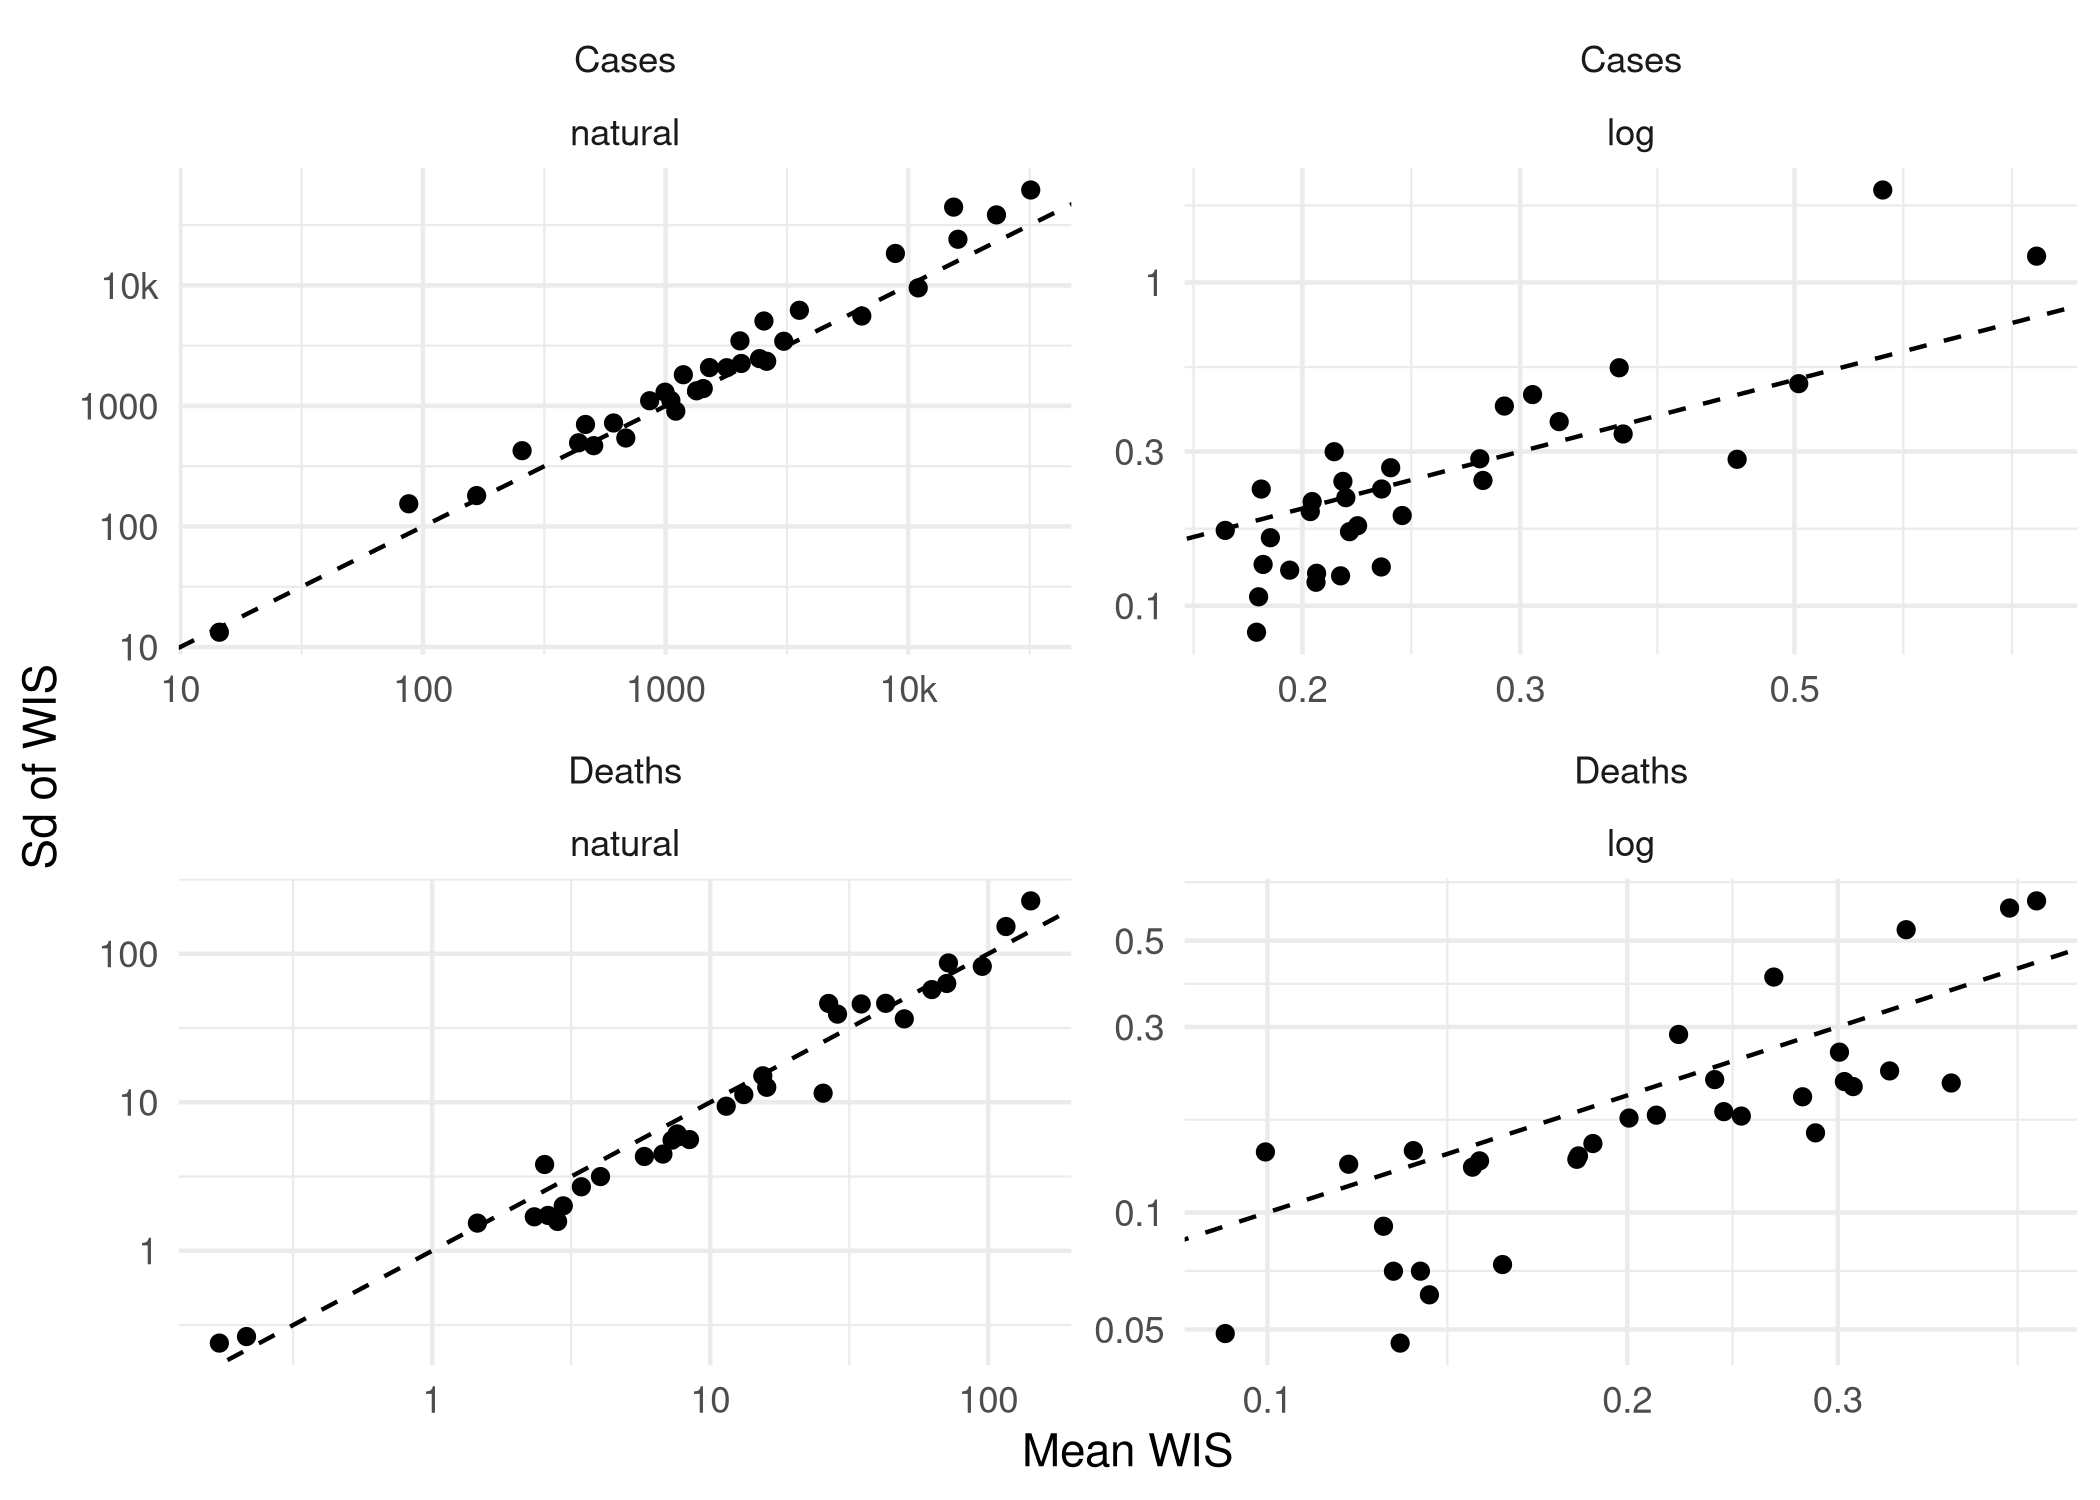
\includegraphics[width=0.9\textwidth]{output/figures/HUB-sd-vs-mean-scores.png}
%    \caption{CAPTION}
%    \label{fig:HUB-mean-sd-scores}
%\end{figure}

%\begin{itemize}
%    \item idea of scores on logged data: interpretation as a measure of relative improvement, just as when you log the absolute error
%\end{itemize}

%\paragraph{What's there in the literature}

%\paragraph{Current problems / questions about scoring an epidemiological setting}
%probably narrow down to the ones we really want to discuss%
%There are limitations with what we can do with scores on a natural scale and open questions whether we can do these things on a log-scale and also whether a log-scale might be inherently more appropriate
%\begin{itemize}
    %\item Can't really model score on a natural scale as errors are heavily skewed. Is there a way to model scores to get insight about different factors that systematically influence scores
 %   \item make a plot somewhere that shows the distribution of scores
  %  \item Maybe epidemiological forecasts are inherently better suited to be scored on an absolute scale due to the multiplicative nature of processes (related to over-prediction > under-prediction)? Does the log-scale imply we are scoring the growth rate? 
   % \item unclear what trade-offs of logging / not logging are
    %\item what score (log, not log) matches closest what our intuition (or policymakers) think is good? 
    %\item are we better at forecasting deaths than cases? --> relative measure would help
    %\item There exists confusion about what can be done to a score in general (e.g. people want to take the median, which they shouldn't) %maybe don't add as an extra point
%\end{itemize}


%\paragraph{Over- and under-prediction}
%If we want to keep this in, we could: 
%\begin{itemize}
%    \item Check whether there is actually a problem with over-prediction and under-prediction in the Hub. This could be the case because we are most interested in certain scenarios in which this might arise. 
%    \item Discuss this in light of Johannes' analysis of how the decomposition of WIS values differs if the data are skewed
%    \item compare this to the PIT-value-like relative bias scores we used for the German / Polish paper, which capture a relative tendency to over- or under-predict, rather than absolute penalties. 
%\end{itemize}


%\section{Modelling scores}
%\paragraph{Motivation} Alternative is to use summary measures or pairwise comparison, which becomes cumbersome for many dimensions. 

%\paragraph{caveats, practical limitations}
%\begin{itemize}
%    \item What kind of transformations can we do? Propose random effect models
%    \item is there anything we can't do? 
%    \item How does logging change the error distribution? On the natural scale, you have huge outliers. What's the appropriate error distribution to use? confidence intervals. Maybe we can only say something about the effects
%\end{itemize}


%\paragraph{Optional: Application to data from the Euro-Hub}
%Also: what, empirically is the distribution of errors? 